\documentclass[10pt,twocolumn,letterpaper]{article}

\usepackage{iccv}
\usepackage{caption}
\usepackage{times, graphicx, amsmath, amssymb, subcaption}
\usepackage[]{algorithm2e}

% Include other packages here, before hyperref.

% If you comment hyperref and then uncomment it, you should delete
% egpaper.aux before re-running latex.  (Or just hit 'q' on the first latex
% run, let it finish, and you should be clear).
\usepackage[pagebackref=true,breaklinks=true,colorlinks,bookmarks=false]{hyperref}

%\iccvfinalcopy % *** Uncomment this line for the final submission

\def\iccvPaperID{1341} % *** Enter the ICCV Paper ID here
\def\httilde{\mbox{\tt\raisebox{-.5ex}{\symbol{126}}}}

% Pages are numbered in submission mode, and unnumbered in camera-ready
\ificcvfinal\pagestyle{empty}\fi
\begin{document}

%%%%%%%%% TITLE
\title{Mosaicing Scenes with Vacant Spaces}

\author{Meghshyam G. Prasad and Sharat Chandran\\
Dept of Computer Science \& Engineering, \\
Indian Institute of Technology Bombay\\
{\tt\small \{meghshyam, sharat \}@cse.iitb.ac.in }
% For a paper whose authors are all at the same institution,
% omit the following lines up until the closing ``}''.
% Additional authors and addresses can be added with ``\and'',
% just like the second author.
% To save space, use either the email address or home page, not both
\and
Michael S. Brown\\
School of Computing, NUS, Singapore\\
{\tt\small brown@comp.nus.edu.sg}
}

\maketitle
%\thispagestyle{empty}


%%%%%%%%% ABSTRACT
\begin{abstract}
  This paper focuses on a method to construct panoramas captured from
  a quadcopter that consists of scenes with significant regions of
  vacant spaces.  These vacant spaces yield little to no features to
  match input images making them challenging for existing
  mosaicing techniques.  

  We describe a framework that is able to handle this unique input by
  leveraging the availability of the inertial measurement unit (IMU)
  data from the quadcopter that is synchronized with the input images.
  Specifically, our method uses the accompanying IMU data to select a
  subset of images that contain interesting scene content. When this
  subset contains no vacant space, the subset results in an
  appropriate panorama; however, with white spaces, the subset is
  partitioned into multiple clusters, again using the IMU data.  These
  subsets can now be stitched into a series of mini-panoramas; the
  gaps between these mini-panoramas represent regions of featureless
  spaces in the scene.  We once again use the IMU data together with
  coarse stereo reconstruction to determine appropriate portions of
  the images to complete the panorama. We demonstrate the efficacy of
  our approach on a number of input sequences that cannot to be
  mosaiced by existing methods.
\end{abstract}

%%%%%%%%% BODY TEXT
\section{Introduction}

Finding features and using them to align images to construct wide field
of view panoramas is one of the success stories of
computer vision.  Virtually all recent consumer cameras have this
technology embedded.  The success of these methods relies significantly on
finding common features in the images that can be used to established the
 appropriate warps to register the images together.

There are scenes, however, that consist of image content that makes this
challenging.  One situation is when scene patterns and texture are repeated.  
This can make it challenging for matching to find appropriate matches.
%Figure 1 shows an example of this.
A more serious situation is when a scene area simply
does not contain features.  This sort of situation occurs in a variety
of situations such as paintings in an art exhibition, or posters in an
auditorium.  Fig~\ref{fig:teaser} shows an example of this case.

The goal in this paper is to create panoramic images of scenes that contain
`vacant spaces'.  Vacant spaces occur when there are large homogeneous regions in 
the imaged scene that have no features.   This results in scene regions that
have no matches and therefore cannot be aligned using traditional mosaicing methods.

\begin{figure}[t!]
  \centering
  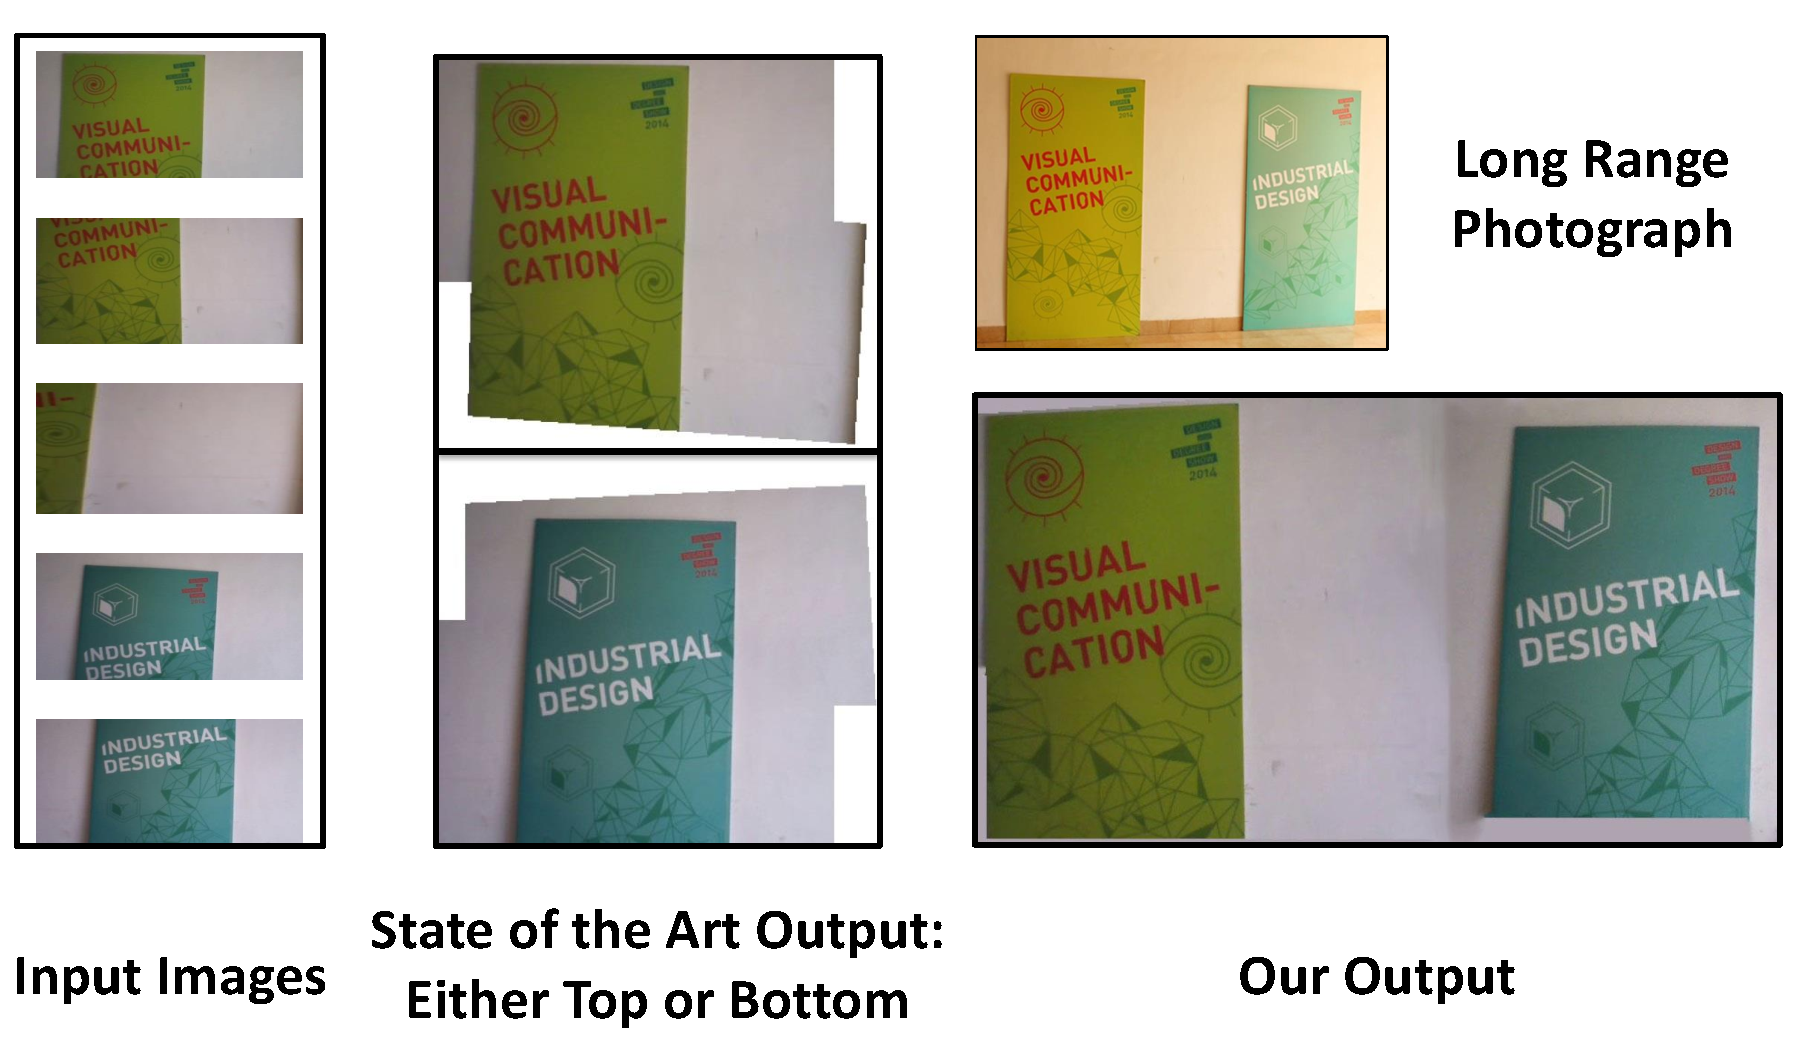
\includegraphics[width=0.57\textwidth]{figures/teaser.pdf}
  \caption{ \label{fig:teaser} The long range photograph of a scene when probed
    by a quadcopter results in the input images shown on the left.  The
    state of the art methods (middle column) are unable to make a mosaic because the
    vacant space (third picture on the left) does not seem to have any
    matchable features with subsequent input images.
    % situation in which dead space exists between large pictures (here,
    % two poster boards). The input images (second column) show parts of
    % the imagery obtained. Even if each of the images of the two
    % individual posters can be stitched together (third column), the
    % state of the art method encounter the dead space and is unable to
    % make a complete mosaic.  It outputs either the first poster or the
    % second, but not both together.  Our method (last column) succeeds
    % since the imagery is acquired using a quadcopter that has
    % positional information
    }
\end{figure}

{\bf Key Idea} We propose to solve the vacant space problem by using
an inexpensive off-the-shelf flying device, such as a quadcopter which
can be assumed to contain an inertial measurement unit (IMU) that has
positional information time synchronized with an input video.  The
proximity relationship that the resultant images have can be used to
significantly reduce the search space in finding matches.  Further,
the proximity relationship also allows, in principle, to vary the
parameters involved in feature selection. For example, if there is
reason to believe that two images are adjacent horizontally, one can
choose to adjust thresholds in feature matching algorithm to hunt for
otherwise elusive matching pairs.

We note that positions can be also made available in other devices
such as smartphones.  An autonomous programmed quadcopter, however, is
particularly enticing because of its ability to fly to areas that are
accessible to the human eye, but inaccessible for the
human to reach.  Such areas do not lend themselves easily to high
quality images.


{\bf Contributions} The main technical contribution of this paper is
that it improves the state of the art in mosaicing.  We assume that
the imagery is acquired by a quadcopter for the reasons mentioned
above. Sending a battery of images from a quadcopter to an image
mosaicing algorithm such as Autostitch
incapacitates the algorithm because of the sheer number of
images. Sending a sampled version of images to a manageable number $N$
of images, with $O(N^2)$ possible areas to match for features, also
does not work since the sampled image contains vacant space.  In this
paper, we use positional information that lends itself to a graceful
$O(N)$ algorithm.  A sample result of our approach is shown in
Figure~\ref{fig:teaser}.  Other results are available in the
experiments section and also in the supplementary material.

%{\bf Limitations} 
In this paper, we assume that the
scene lies on a planar surface, or can be deemed to lie on a planar surface. The
standard homography computation is still not possible because of the
vacant spaces. To overcome this, we reduce the mosaicing problem to
the stereo problem and are thus able to complete the panorama.


The rest of this paper is organized as follows.  In the next section,
we discuss related work.  Subsequently we describe the main steps in
our process, and justify the process in Section~\ref{sec:results} with
experimental results.  The data and the code will be made available
later, but as of now it is available in the supplementary material.
The final section discusses future work.

\section{Related Work}

Panoramic image stitching (alternatively, image mosaicing) is a
well-studied problem in the field of computer vision.  Representative
works include~\cite{Milgram1975}, \cite{Milgram1977}, \cite{Capel},
\cite{Szeliski1997} \cite{Brown07} \cite{Brown03}.  A full discussion
on related works is outside the scope of this paper, readers are
referred to~\cite{Szeliski05imagealignment} for an excellent survey.
Given the maturity of this area, there are various freeware as well as
commercial software available for performing image stitching; most
notable are AutoStitch \cite{autostitch}, Microsoft’s Image
Compositing Editor \cite{ICE}, and Adobe’s Photoshop \cite{photoshop}.
All of these methods are based on a similar strategy of finding
features in each image, matching these features between images, and
then computing pairwise image warps to align them together.  A global
bundle adjustment is often applied to globally refine the alignment.
All of the aforemention methods assume the imaged scene is planar or
that the camera has been rotated carefully around its center of
projection to avoid parallax.

% MSB - I'm not sure how any of these are relevant to what you are doing
%There has been work to address non-planar scenes.  Gao et al. \cite{Gao} have
% used the concept of ``Dual Homography'' to stitch non-planar patches in images. Lhuillier \etal \cite{Lhuillier}
%have successfully stitched images with motion parallax \ie relief
%mosaics, using joint view triangulation.  Acha \etal \cite{Acha} have
%aligned dynamic scenes using the notion of ``dynamics constancy''.

% MSB - I'm also not sure how this is relevant to what you are doing
%Agarwala \etal \cite{Agarwala2006} have used Markov Random Field (MRF)
%optimization for stitching a relatively sparse set of images captured
%using handheld still camera which is moved along the scene.
Brown \etal \cite{Brown05} have used a new type of invariant features
located at Harris corners in discrete scale-space and oriented using a
blurred local gradient for stitching. Eden \etal \cite{Eden} were
able to stitch images with large exposure difference as well as large
scene motion into single HDR quality image without using any
additional camera hardware.

All of the image mosaicing methods work only when there is a
``intersection'' in feature space of images to be stitched. When there
are ``gaps'' (either physical or due to lack of features) between
images to be stitched it is not clear how to perform the stitching. In
this paper, we discuss how to use the available IMU data that
accompanies our input images to help overcome these problems.

%Peleg et al. \cite{Peleg} have used similar concept to create Stereo Panorama
%with a single camera.

\section{Methodology}

% MSB - if you do not demonstrate any example of a scene lying on more than
% one plane, you should not list it as a goal.  All goals listed must be demonstrated.
The goal of this paper is to compute a panorama of a scene lying on
planar surface that has regions of vacant spaces.  A schematic for
this problem is shown in Figure~\ref{fig:schematic}.

\begin{figure}[h!]
  \centering
  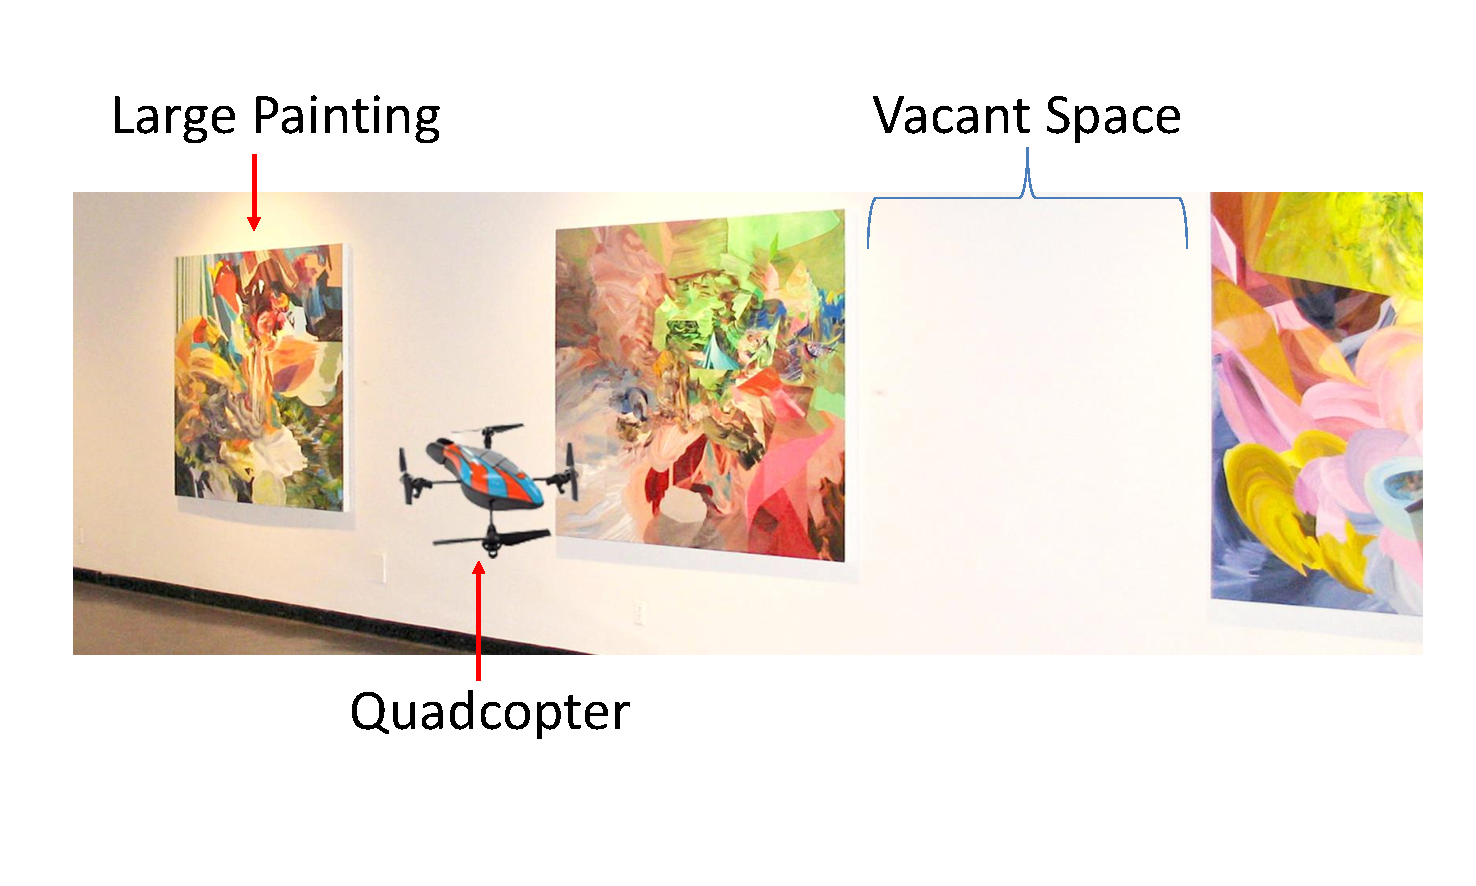
\includegraphics[width=0.49\textwidth]{figures/indoor}\\
  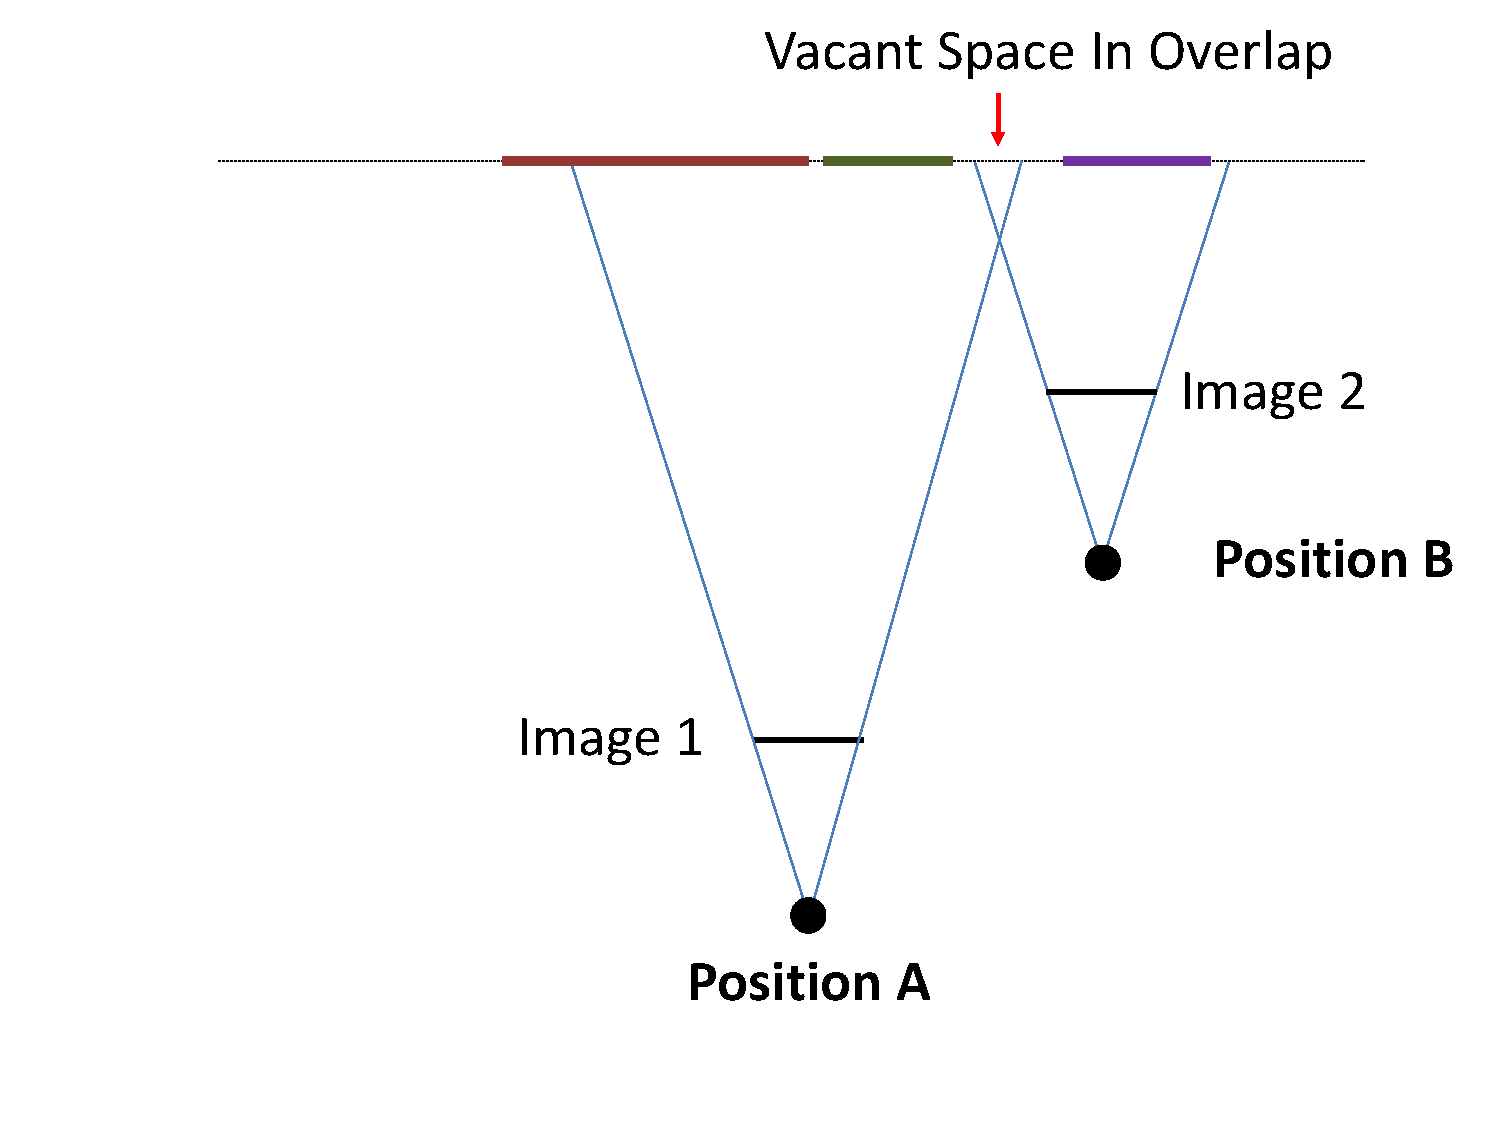
\includegraphics[width=0.49\textwidth]{figures/stereoOverlap}\\

  \caption{ \label{fig:schematic} Problem definition. (Top) Vacant spaces
    are encountered in various scenes.  When individual portions are
    captured by a quadcopter, how does one create the complete mosaic
    given that common features are either not available, or
    confusing?\\
    (Bottom) Simplified reduction of the problem to a geometrical structure.
  }
\end{figure}    

% MSB - Mashup, what does this mean.  It isn't a technical term.
The method adopted is pictorially depicted in the overview shown in
Figure~\ref{fig:workflow} and is described in detail later on.  In
brief, we systematically acquire a video of the scene, reduce the large
number of images into a manageable number, and finally combine the
images acquired from different positions into a mosaic.

\begin{figure}[h!]
  \centering
  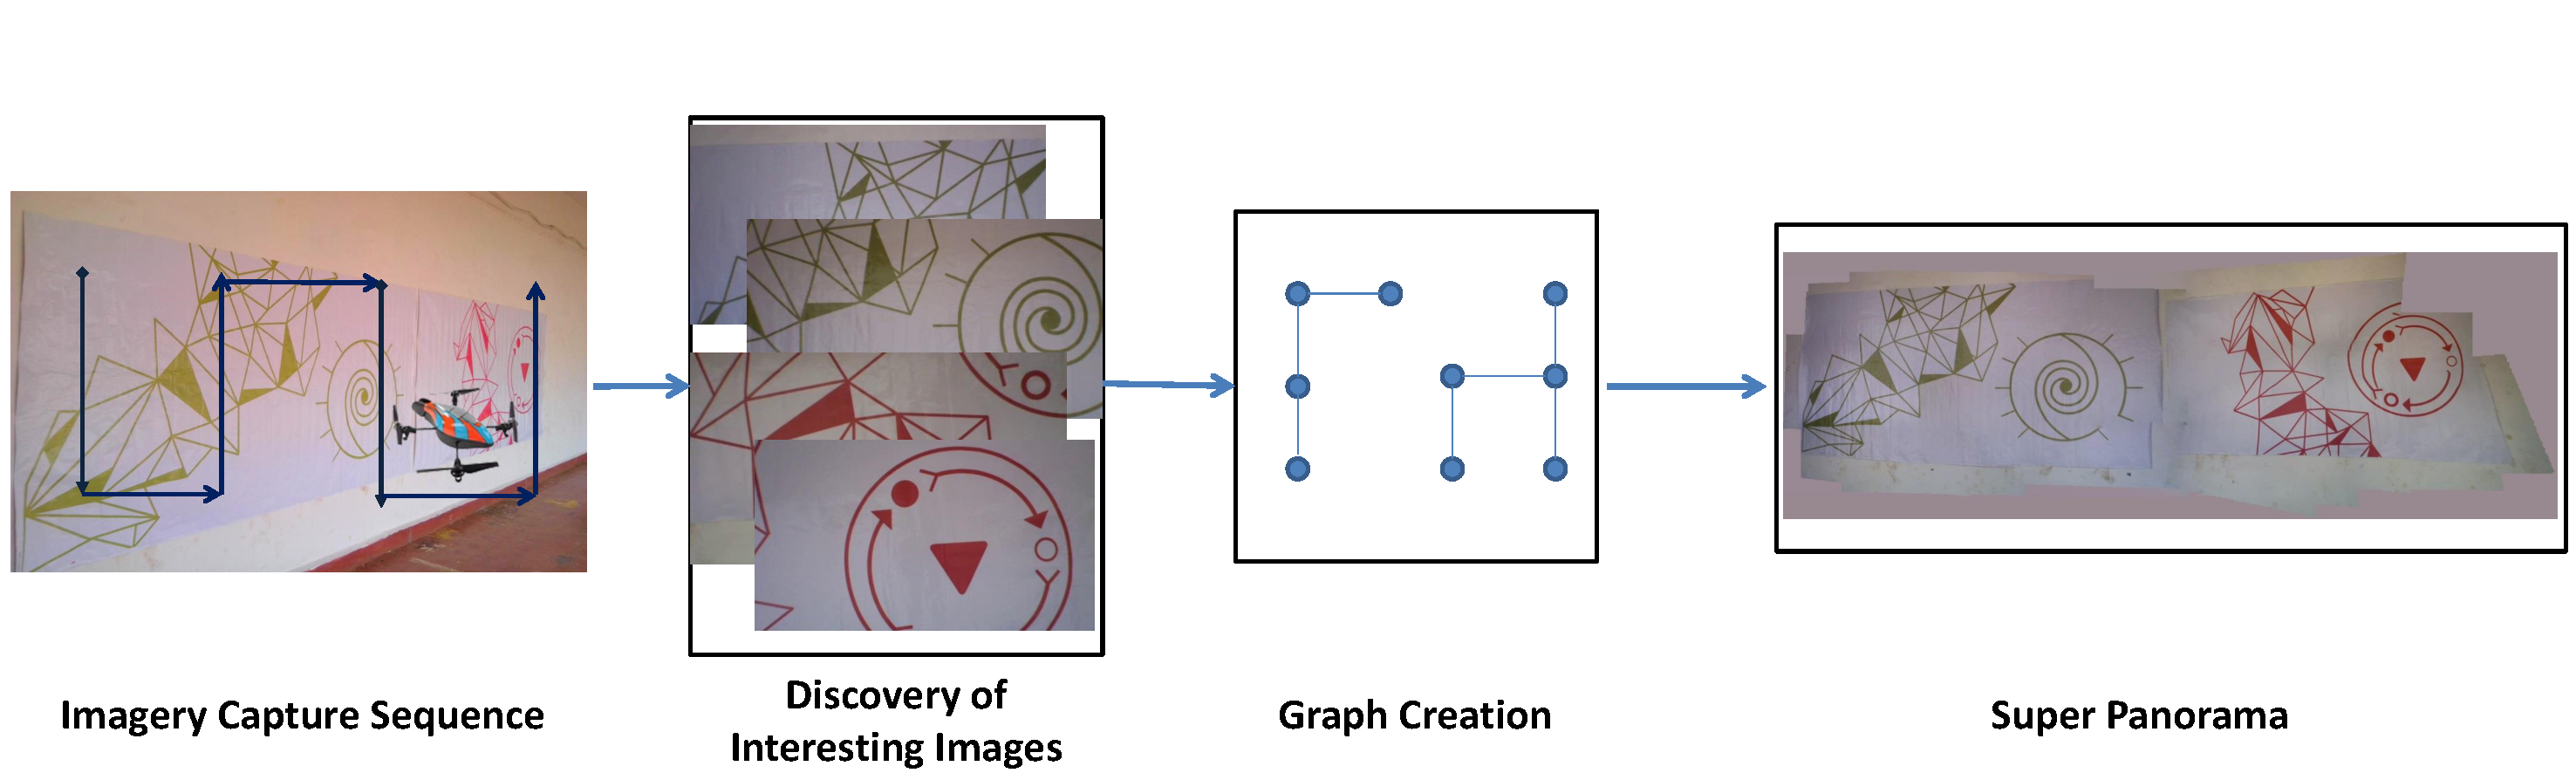
\includegraphics[width=0.49\textwidth]{figures/Workflow} 
  \caption{ \label{fig:workflow} Overview: Input imagery is
    systematically acquired (top left) by a quadcopter.  In the next
    step, interesting images are found by clustering the video into
    regions based on positional data.  A graph is constructed using
    proximal images. For each connected component in a graph, standard
    stitching techniques are used to create mini-panoramas which are
    then joined together into super panorama 
    again using IMU data.}
\end{figure}    


\subsection{Video acquisition}
We first despatch the quadcopter to as close to the scene as
possible. The corners of a rectangular area of interest is provided to
the quadcopter, and it is programmed to traverse the area in a snake
like raster scan fashion.  There are various control aspects involved
in sending a quadcopter; in outdoor areas, the quadcopter is impacted
by wind and it might lose its way.  The control aspects of the
quadcopter is beyond the scope of this paper.

The quadcopter returns with a video of the scene.  Any short video of
about a minute or more when given to a stitching program such as
Autostitch overwhelms the programs rendering it unusable. In the rest
of this section, we use Autostitch to indicate state of the art
stitching programs such as Autostitch, Photoshop, etc.

\subsection{Acquiring interesting images}
\label{sec:selection}
% MSB - any citation to standard albumization?
Our goal in this step is to reduce the amount of input data and
produce a set of interesting images.  In other words, we wish to
convert a video into an album of images.  The key difference between
our problem and standard albumization \cite{Aner, Lee} is the use of 
positional information.  A standard quadcopter has an Inertial
Measurement Unit (IMU) that, after calibration, can give accurate
information of positions.

%It is to be noted that this information can be quite incorrect.  
Using this it is possible to cluster the images, and sort the images
into an $m\times n$ grid.  (Occasionally we have encountered outlier
situations and thus erroneous positional information.  Thus we believe
standard vision-based clustering method can be used to either drop
frames, or to correctly include frames based on image content.)  The
number of cluster centers is automatically determined using the
agglomerative bottom up hierarchical clustering method \cite{Lior}, with the
additional requirement that the whole scene (represented by the
positional data) is covered.  

{\bf Clustering Details} We assume that each IMU data position
corresponds to an image of definite fixed dimensions.  Consider each
position of the IMU data to be a leaf node. Two nodes are greedily
combined based on the closest Euclidean distance, and replaced with an
internal node.  The position of the internal node is set to be the
centroid of the two nodes, and each internal node now corresponds to a
virtual image taken by a virtual quadcopter.  The algorithm
recursively merges all the nodes till we end up with a root.  In the
next phase, we proceed top-down and level by a level to find the
cluster centers.  A set of nodes is considered for being the output as
cluster centers if the union of these nodes completely cover the
scene. From the bottom-up construction, it is clear that the root will
represent a single position, and thus a single image and most likely
will not cover the scene.  At the other extreme, the set of all leaf
nodes \emph{will} cover the scene.  The top-down algorithm proceeds
top-down and finds the minimal set of nodes which cover the scene.
Once cluster centers are found, we pick the leaf node which is closest
to the cluster center to find a real image.
This process is pictorially described in
Figure~\ref{fig:selection}.


\begin{figure}[h!]
  \centering
  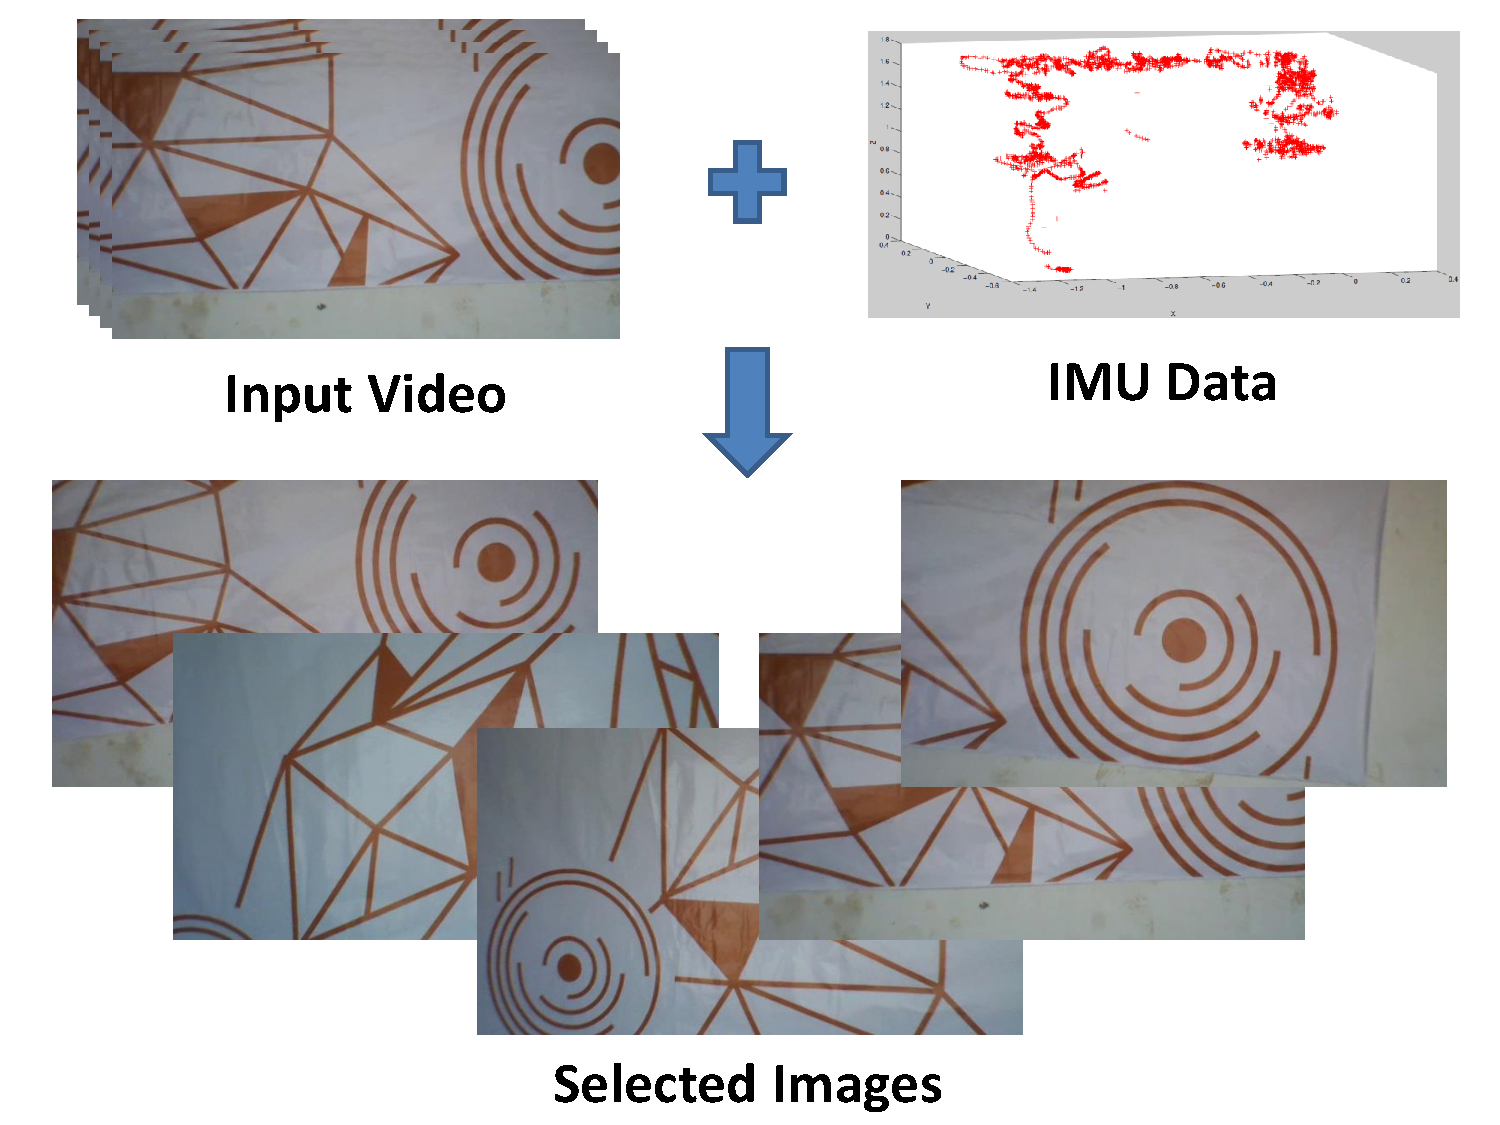
\includegraphics[width=0.49\textwidth]{figures/selection} 
  \caption{ \label{fig:selection} Using IMU data, an image stream is
    transformed into a set of interesting images for purposes of
    panorama creation. }
\end{figure}    

% MSB - what is meant by ``wrong position'', how will the reader know 
% this is relevant to the problem here.  Why not discuss vacant space,
% the message is being muddled? 
In practice, the number of cluster centers for the scenes we have
covered is now within the capacity of Autostitch.  As mentioned in the
introduction, as long as there are sufficiently varying and
``matchable'' features, Autostitch is able to perform a reasonable
result.  However, if there are very few features in overlapping region
of two images, then the output is not acceptable. This situation will
arise when there is vacant space between two pictures.

{\bf Time complexity} Autostitch has not been designed
to use positional information. As a result if there are $N$ input
images, the program has to consider possible matches in approximately
$O(N^2)$ set of areas.  Our program is able to mosaic in an $O(N)$
fashion.

% MSB - There are no details to the clustering, or the "postulating" of edges.
{\bf Spanning Trees}
Specifically, we assume at this point that the interesting photos are
available in the form of a $m \times n$ grid. First, we find SURF
\cite{Bay} features for each image in a grid. Next, we use Best of
Nearest Neighbor matcher (from the OpenCV library) with Random Sample
Consensus (RANSAC) \cite{Fischler1981} to find geometrically
consistent matches between neighborhood images inside grid.  We
create a graph with images being nodes, and add an edge between two
nodes if there are sufficient matches. We have to recall at this point
that if there are ``vacant spaces'' there will not be enough features
for successful matches; the graph will end up with multiple
(disconnected) components.  We next compute multiple spanning trees
for the various components. Given a spanning tree, the center of the
spanning tree is a node from which the distance to all other nodes is
minimal. Next we calculate the homography of each image with respect
to spanning tree center.  Finally, for each spanning tree, we stitch
all pictures using the computed homographies by warping all images
with reference to the image at spanning tree center. The spanning tree is
an $O(N)$ structure. The process is described in
Figure~\ref{fig:graph}.
% above - what homographies. there has been no discussion on how
% warps are estimated from the features. . or even the features used.
% is ransac used?  do you call autostitch.  you can't get away with 
% not discussing this in ICCV.  The paper reads like a high-level
% sketch of an procedure, but lacks technical depth


\begin{figure}[h!]
  \centering
  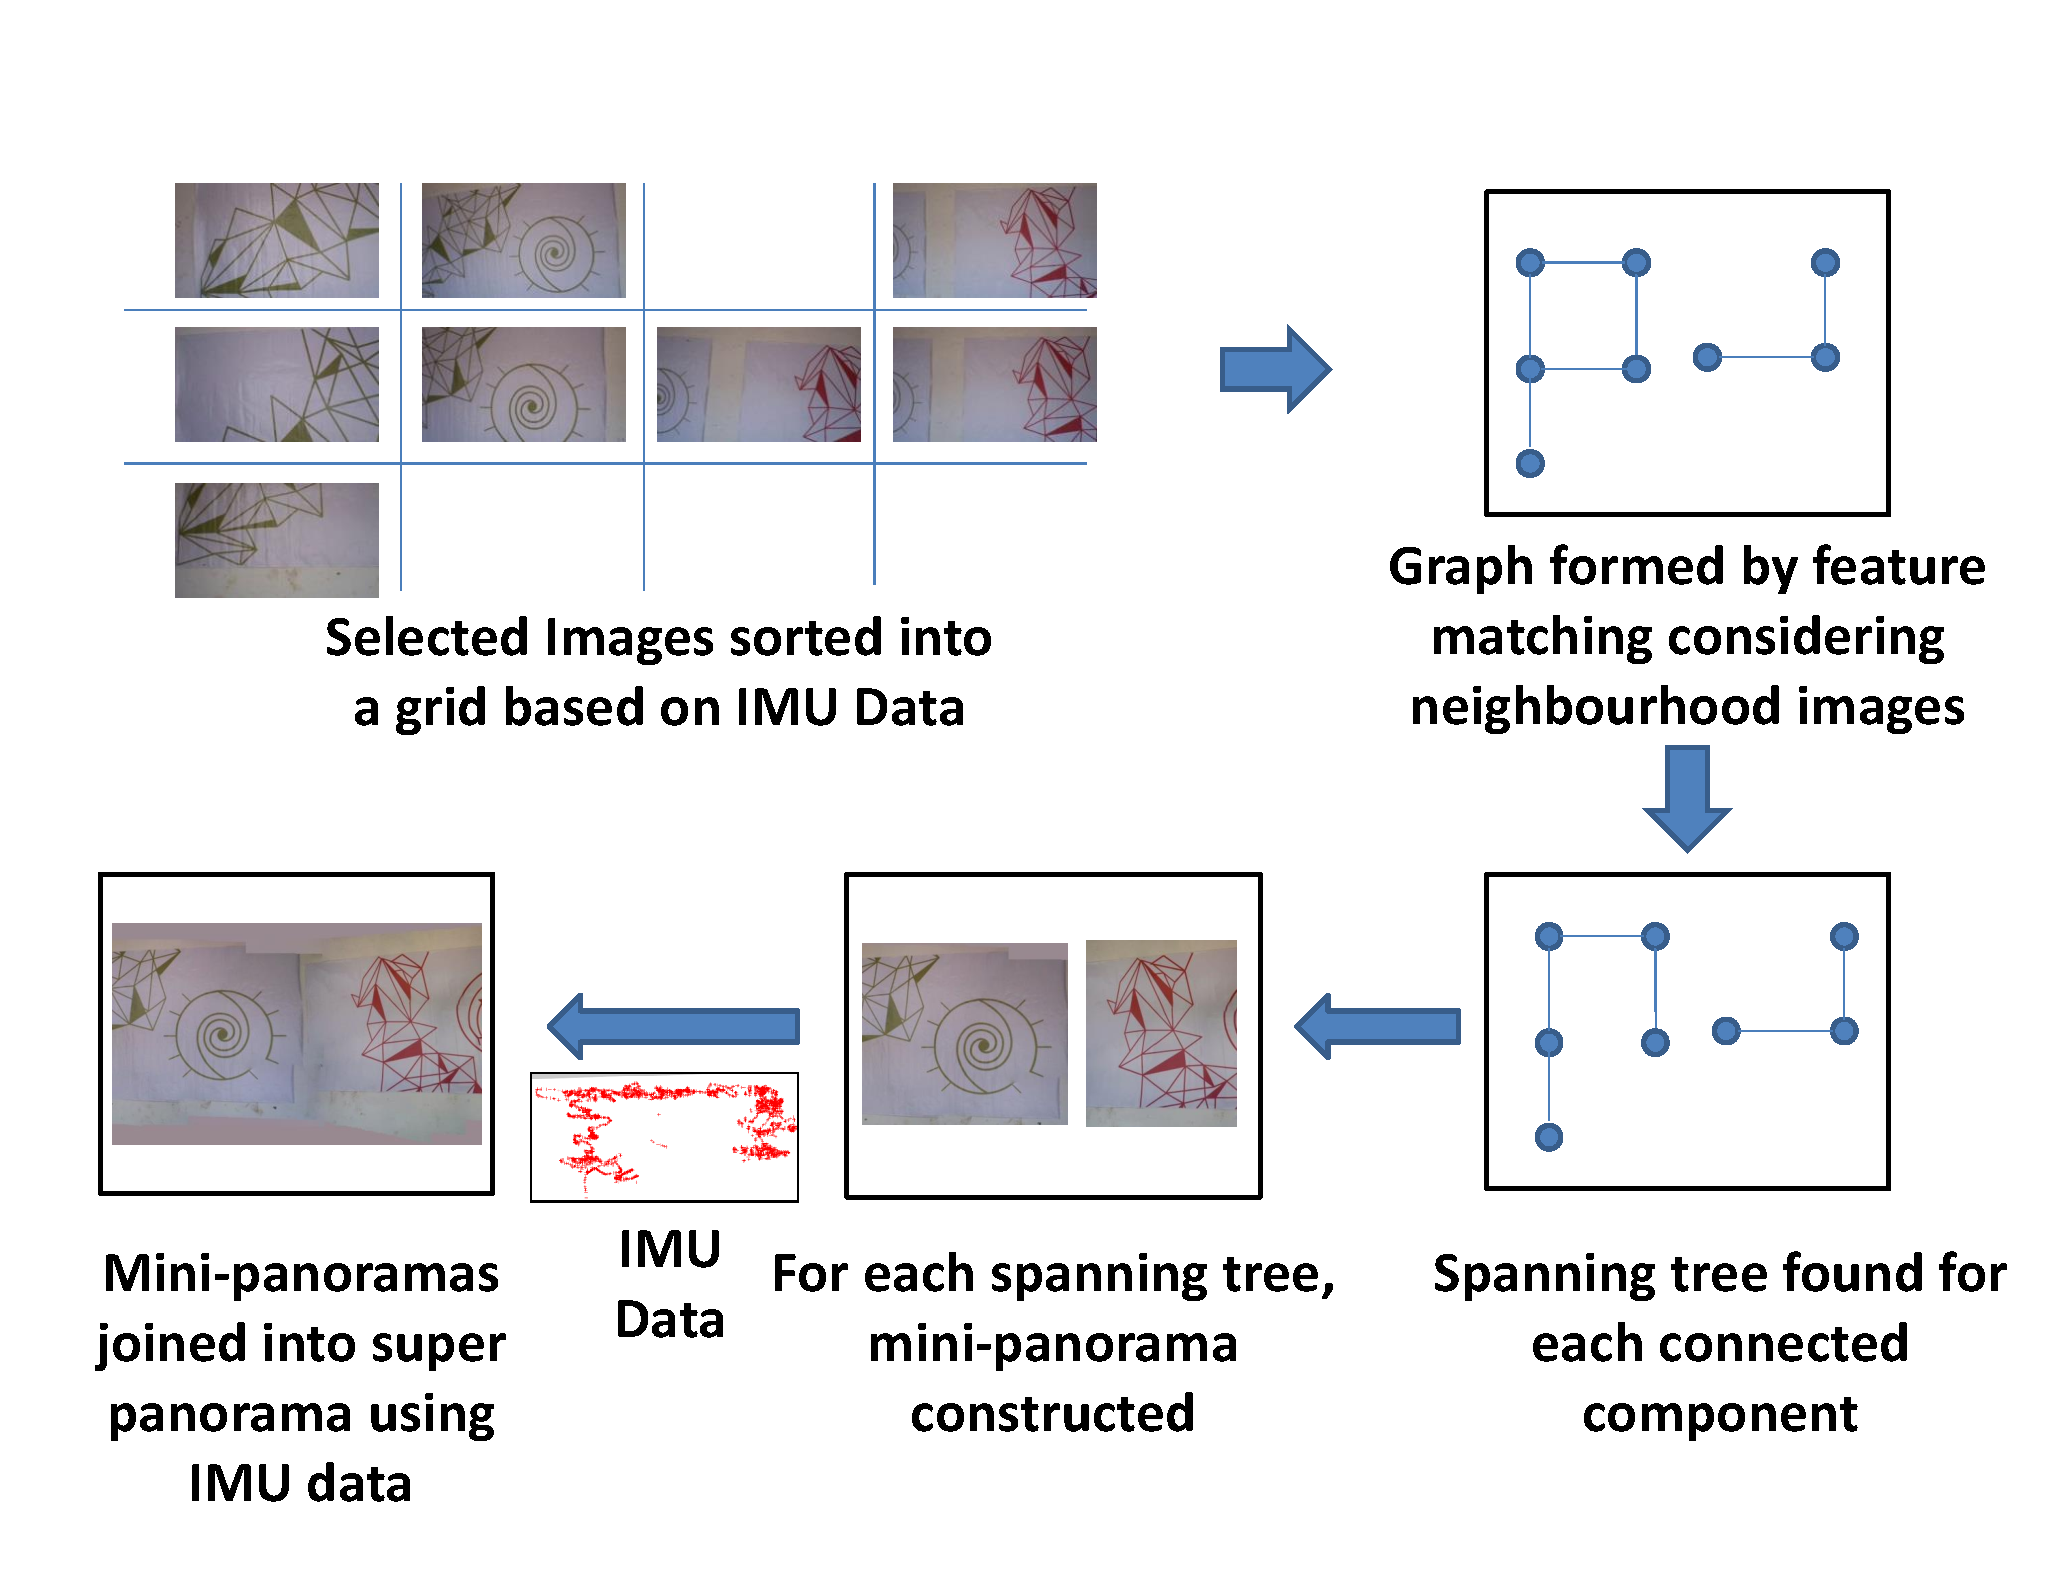
\includegraphics[width=0.49\textwidth]{figures/graphCreation} 
  \caption{ \label{fig:graph} Interesting images acquired are
    segmented and individual (mini-panoramas) are constructed. These
    are then later combined into the desired super-panoramas using IMU data.}
\end{figure}    


\subsection{Super-panoramas}
% MSB - Why do you assume each spanning tree corresponds to a specific depth?
% There is no details to this?  
In this section, we consider the situation when programs like
Autostitch fail.  We assume that the output of the previous step has
resulted in multiple spanning trees where each spanning tree center
corresponds to a specific depth. This is the depth of the center of
the spanning tree, since we have stitched all images by taking the
spanning tree center as a reference.  Individual panoramas for each
spanning tree termed mini-panoramas have been created. A
super-panorama must be created from mini-panoramas; these usually
correspond to different depths for at least two reasons.

First, it is invariably difficult, if not impossible, to control a
quadcopter to be at the exact depth even in indoor scenes.  The
aerodynamics and the thrust produced tends to make the quadcopter
drift.  Second, it might also be necessary to let the quadcopter probe
and come closer to the scene so as to get a ``good picture''.

A super-panorama is done using a two step process. Assume two trees in
the forest corresponding to area A and area B of the scene (see
Figure~\ref{fig:stereo}). 
\begin{figure}[h!]
  \centering
  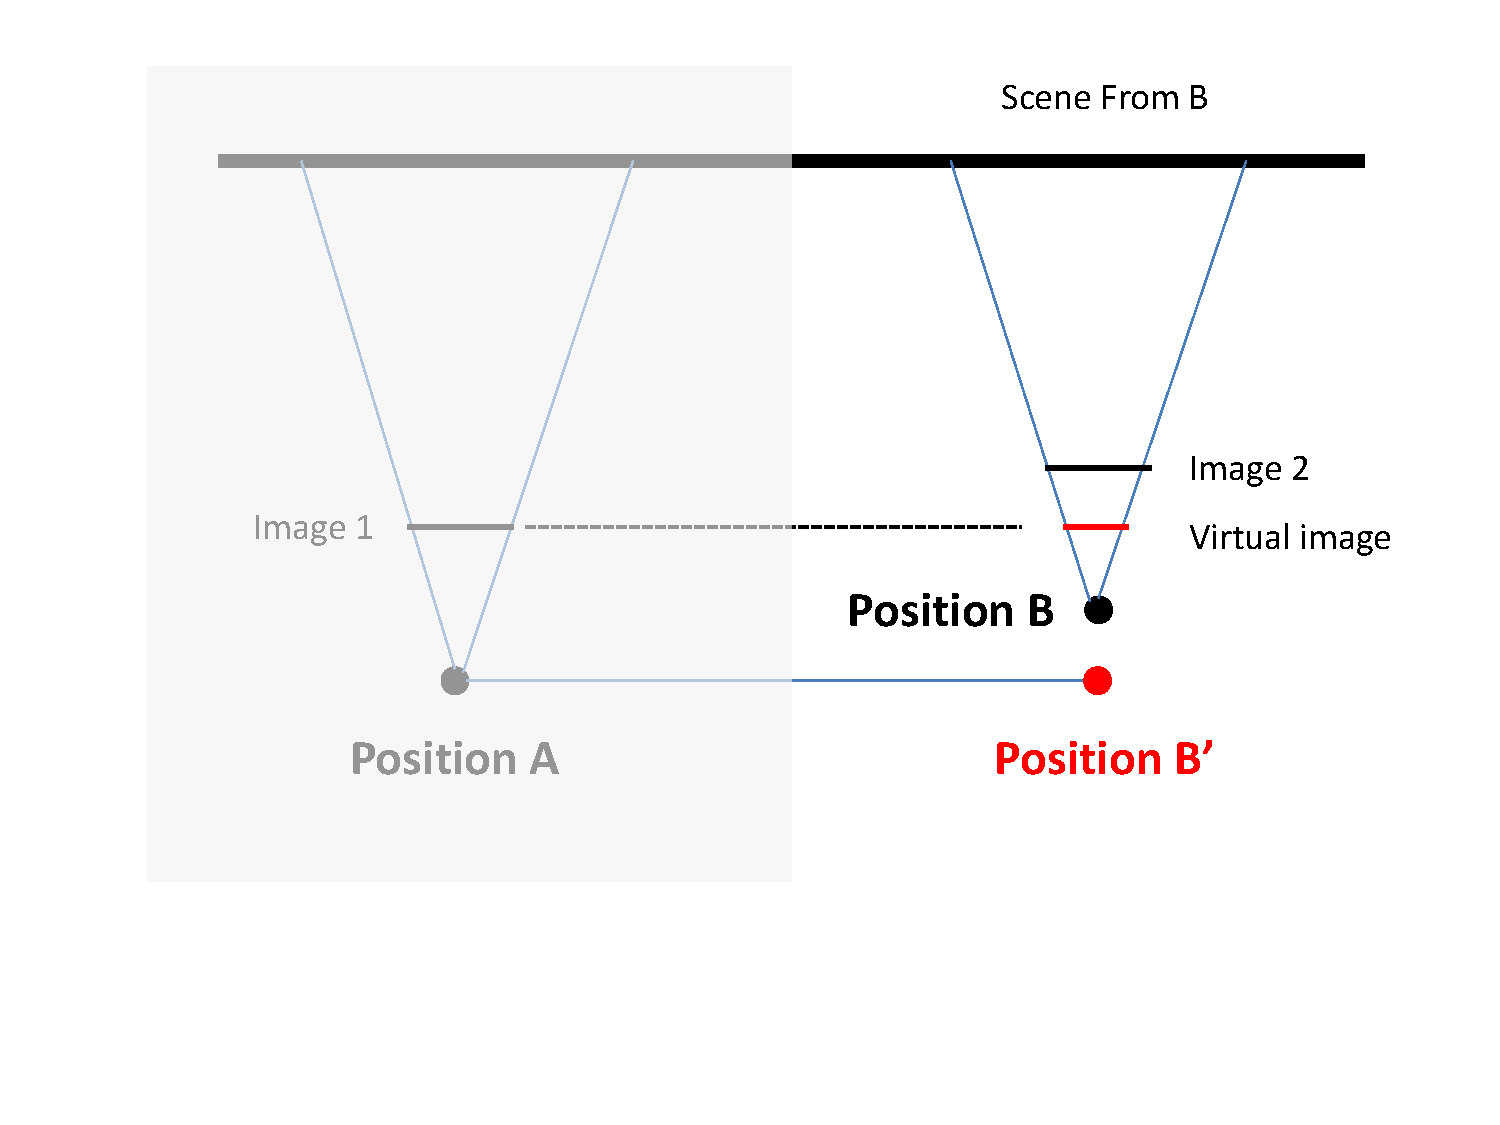
\includegraphics[width=0.4\textwidth]{figures/move} \\
  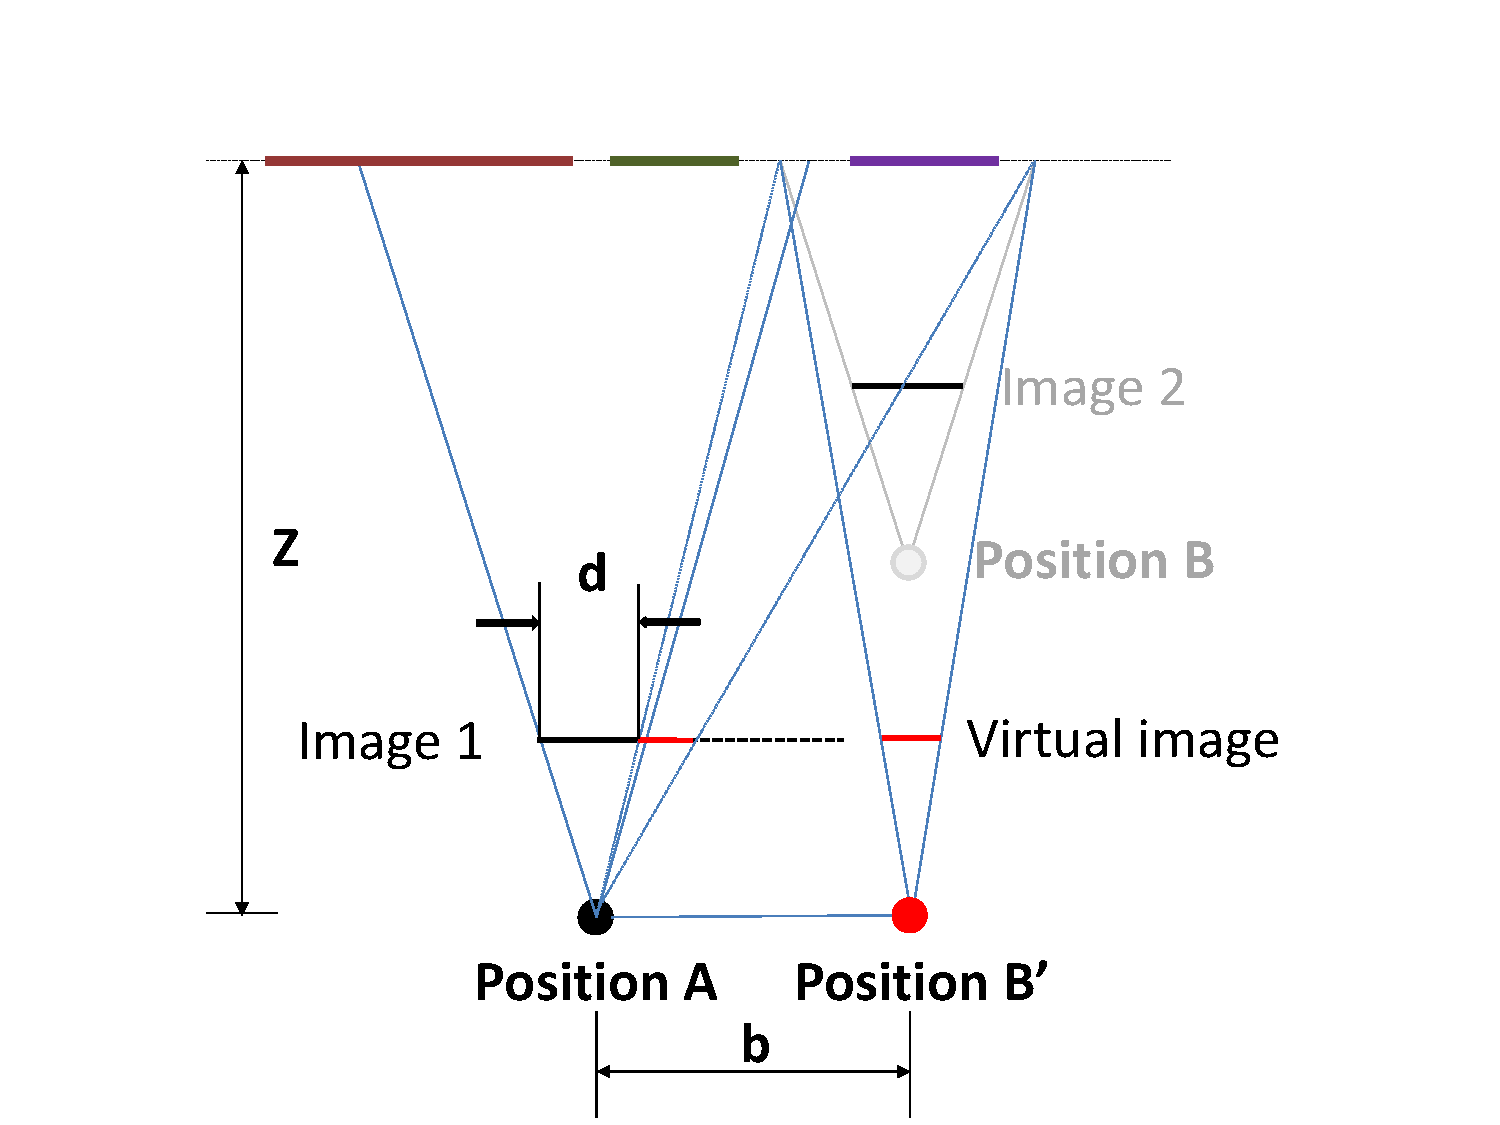
\includegraphics[width=0.4\textwidth]{figures/stereo} 
  \caption{ \label{fig:stereo} Top: The virtual picture as seen from position B'
    is computed using Equation~\ref{eq:moveRelation} from the real picture
    taken from B.  Bottom: Using the disparity, and the baseline width,
  it is possible to depict the composite scene obtained from both A
  and B' (from the view point of A).}
\end{figure}    
Assume that a mini-panorama is created from these two areas, and the
depth of the planar surface from the camera is more for A, than for
B. We then take the mini-panorama image captured at B, and `move' it to
a new location B’ whose depth (from the imaged surface) is the same as
that of A. The resulting image  will be smaller; the images are
related by the equation
\begin{equation}
  \label{eq:moveRelation}
  {\bf \frac{x'}{x} = \frac{Z}{Z'}}
\end{equation}
where {\bf x} (respectively {\bf x'}) represents a pixel location of
the image in B (respectively, B') and 
{\bf Z} (respectively {\bf Z'}) represents the depth of the images
surface from B (respectively, B').

We can now treat the resulting images from A (unchanged) and B’
(computed from Equation~\ref{eq:moveRelation}) forming a stereo pair.
Using the stereo disparity formula we can ``place,'' from the view
point of A, the image captured from B, thereby creating a
super-panorama.

\section{Experiments and Results}
\label{sec:results}

All our experiments have been completed with the inexpensive consumer
quadcopter called Parrot's AR Drone 2.0. We have used the ROS based
ARDrone Autonomy Driver to communicate with the drone. For the
purposes of establishing the ground truth, pictures were taken with a
5 mega pixel camera.

We have implemented our algorithm in C++ using the OpenCV library
(OpenCV 2.4.9). Experiments were performed on a PC with Intel Core i7
processor(@3.4GHz) and 8GB RAM.  The source code to produce
interesting images from a video, and to generate the super-panorama,
as well as the data sets used in this paper will be made publicly
available.


\subsection{Establishing Correctness}

In our first experiment, we wanted to ensure that the selection of
images done was comprehensive.  We sent the drone to recce an outdoor
scene with no dead space. This experiment was conducted in an outdoor
environment. We note here that there were approximately 9000 images in
the raw video.  Autostitch was unable to cope when fed with this large
number. 

One way to produce some sort of mosaic was to simply reduce the amount
of data given to Autostitch.  Figure \ref{fig:uniformsampled_sac3}
shows uniformly time sampled images from complete video.  When these
uniformly sampled images are given to Autostitch or to Adobe
Photoshop, we find (Figure \ref{fig:results_sac3_timesmapled})  that the
results are not satisfactory.

Instead of feeding time-sampled images, we ran our saliency selection
algorithm on the video. Figure \ref{fig:selected_sac3} shows examples of
selected images. Many of the images are similar to the time sampled
version; however, the occasional differences are enough to make
Autostitch work. 

Using only $N=5$ images, the results are shown in
Figure~\ref{fig:results_sac3_timesmapled}.


\begin{figure*}[htb!]
\centering

\includegraphics[width=0.19\linewidth]{figures/sac3/uniform_sampled/1.jpg}
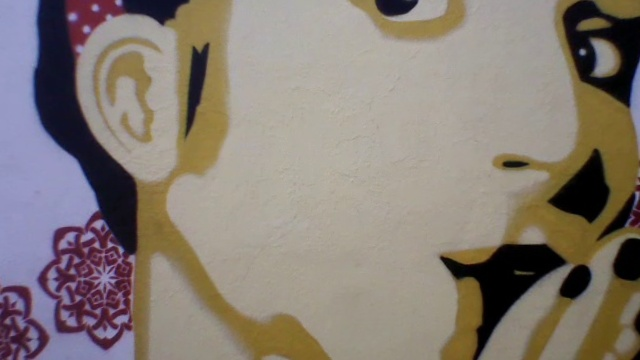
\includegraphics[width=0.19\linewidth]{figures/sac3/uniform_sampled/5.jpg}
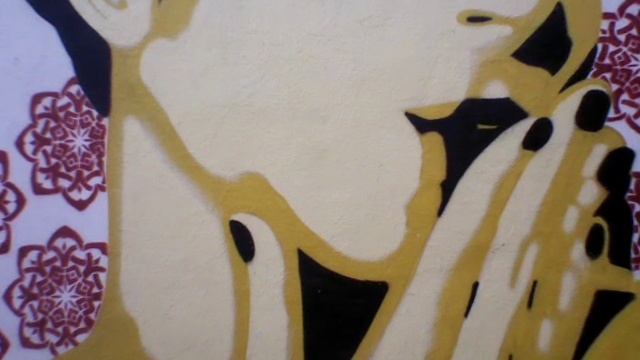
\includegraphics[width=0.19\linewidth]{figures/sac3/uniform_sampled/4.jpg}
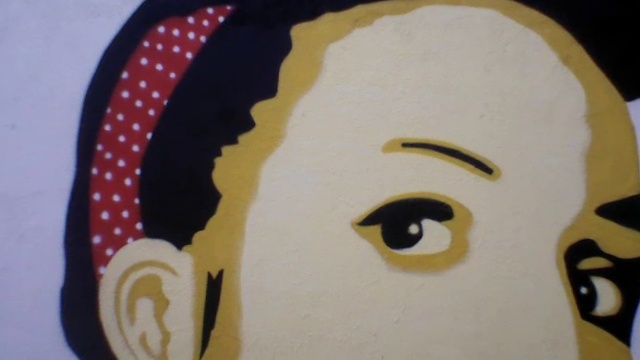
\includegraphics[width=0.19\linewidth]{figures/sac3/uniform_sampled/2.jpg}

\includegraphics[width=0.19\linewidth]{figures/sac3/uniform_sampled/3.jpg}
\caption{Uniformly sampled images from an outdoor video expedition.}
\label{fig:uniformsampled_sac3}
\end{figure*}

\begin{figure*}[t!]
\centering
\begin{subfigure}[b]{0.4\textwidth}
\centering
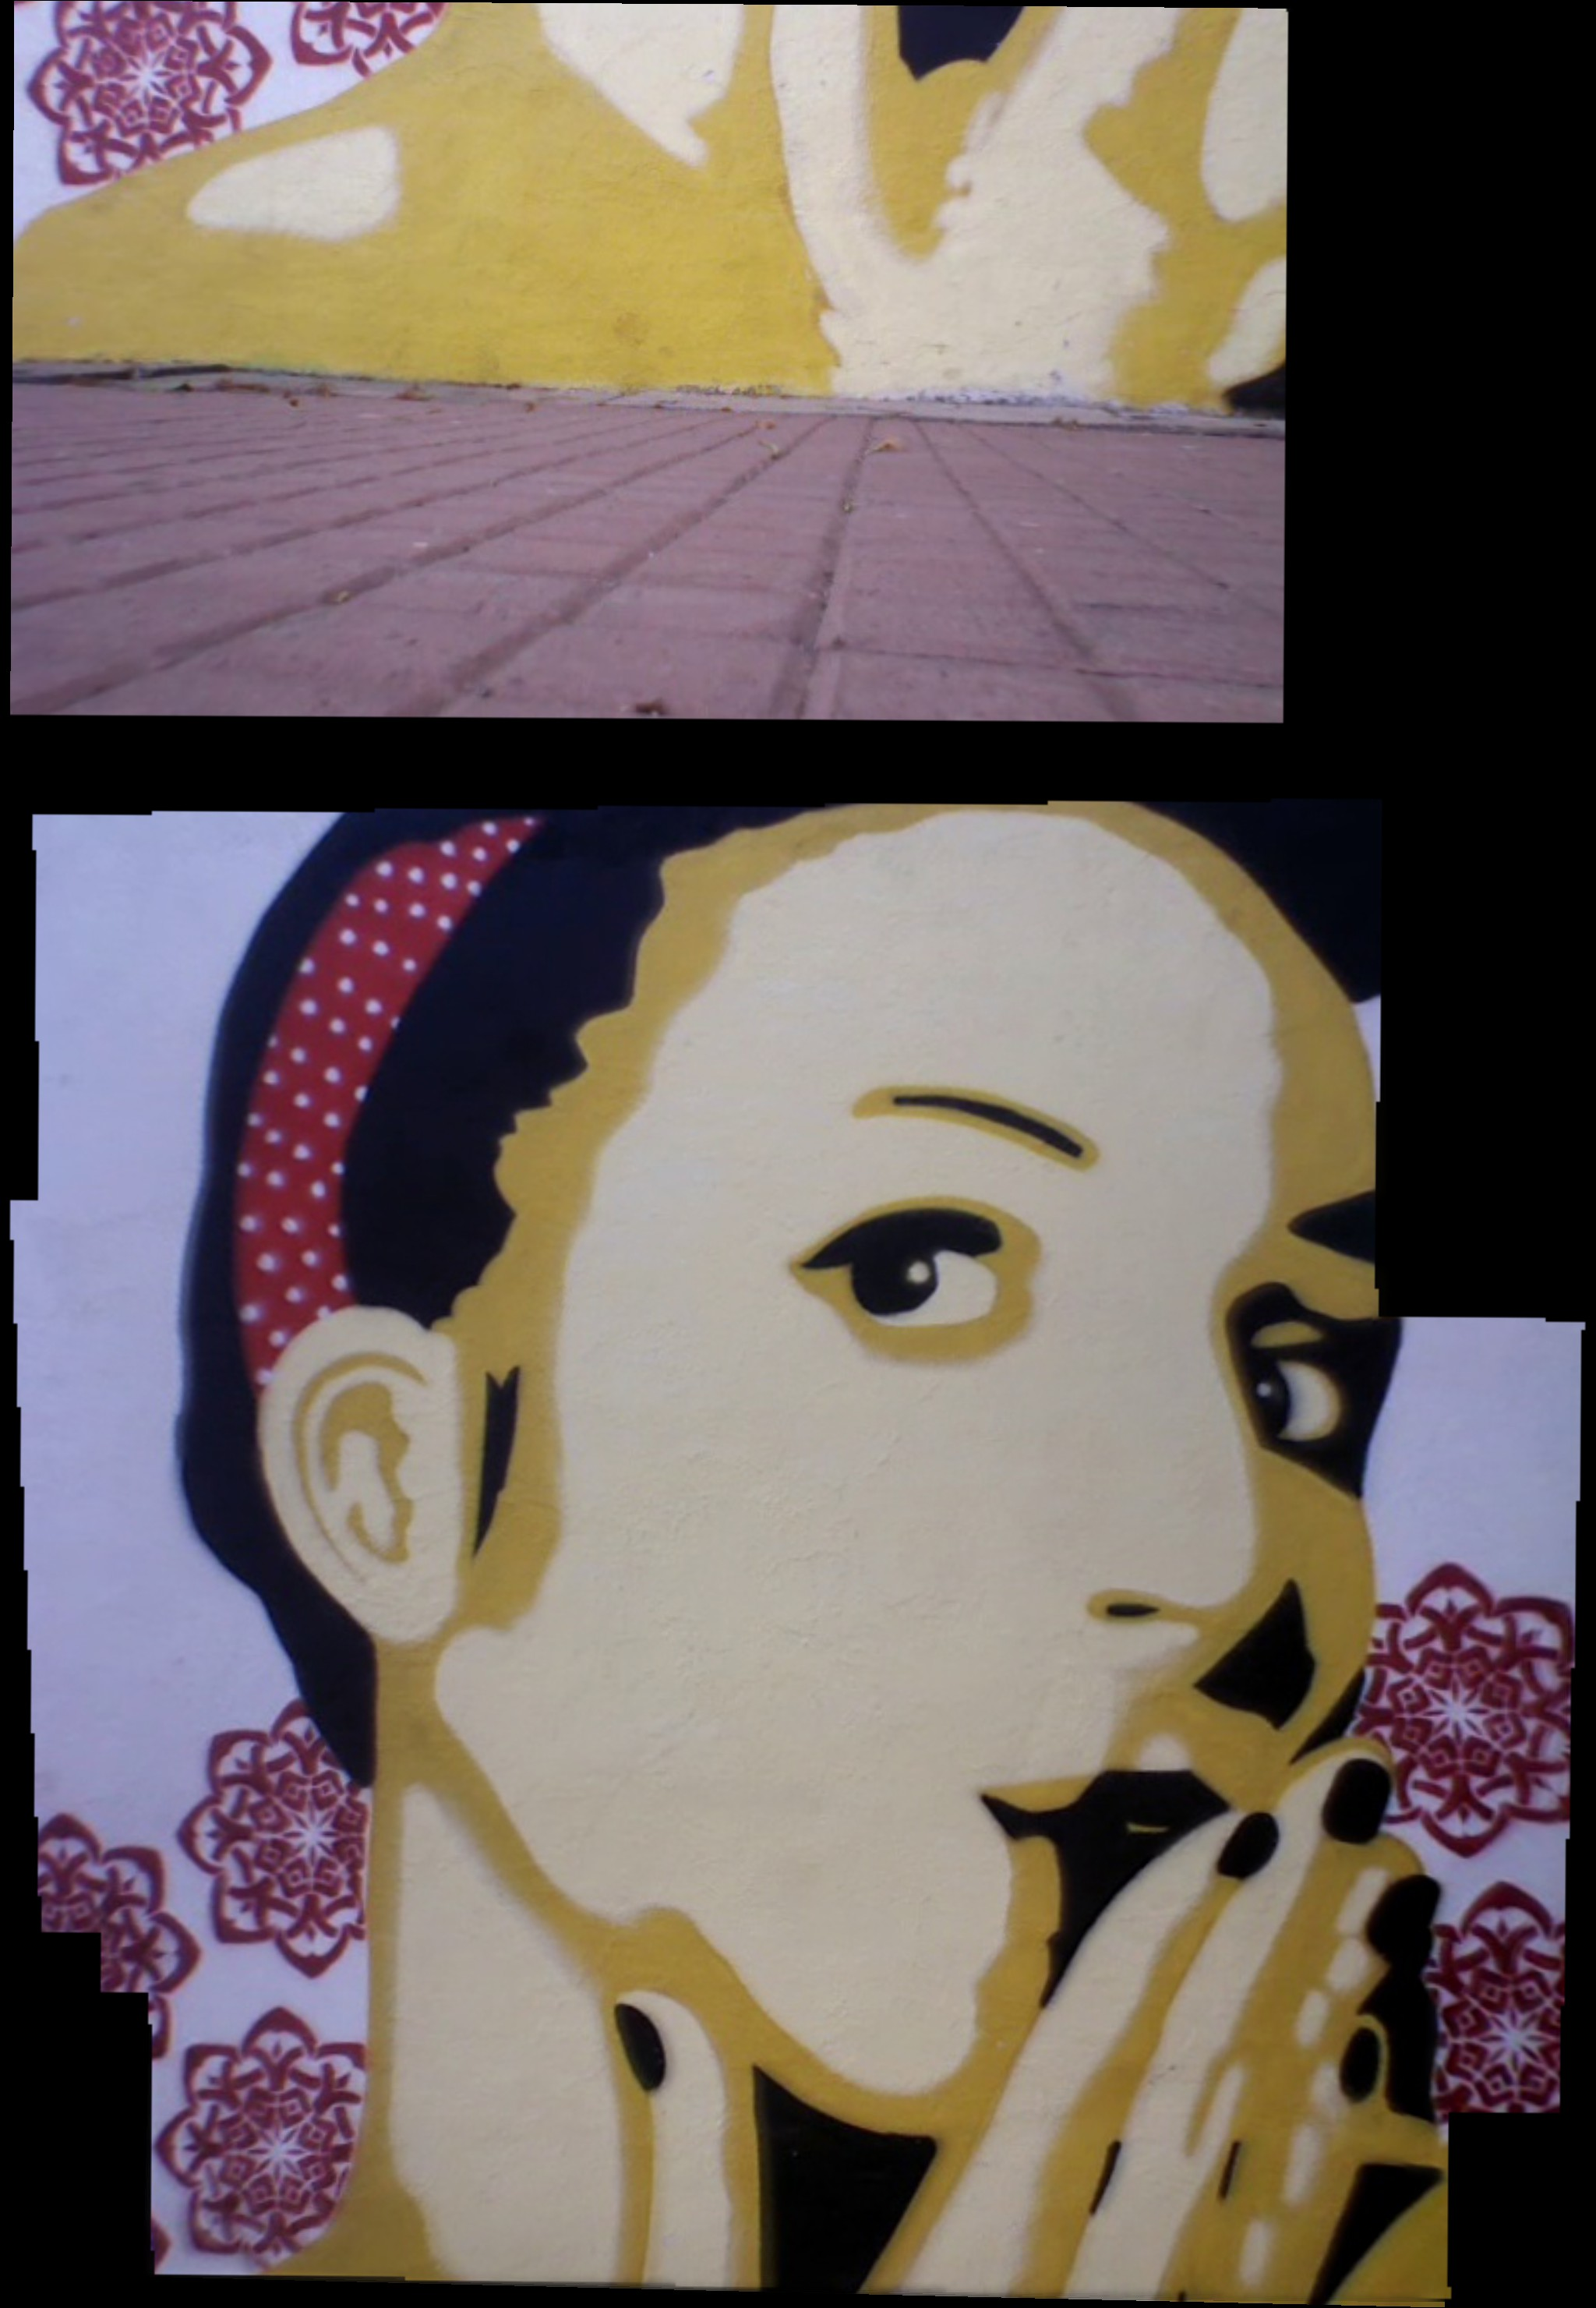
\includegraphics[width=\linewidth]{figures/sac3/uniform_sampled/autostitch.jpg}
\caption{Autostitch Result}
\end{subfigure}
\begin{subfigure}[b]{0.4\textwidth}
\centering
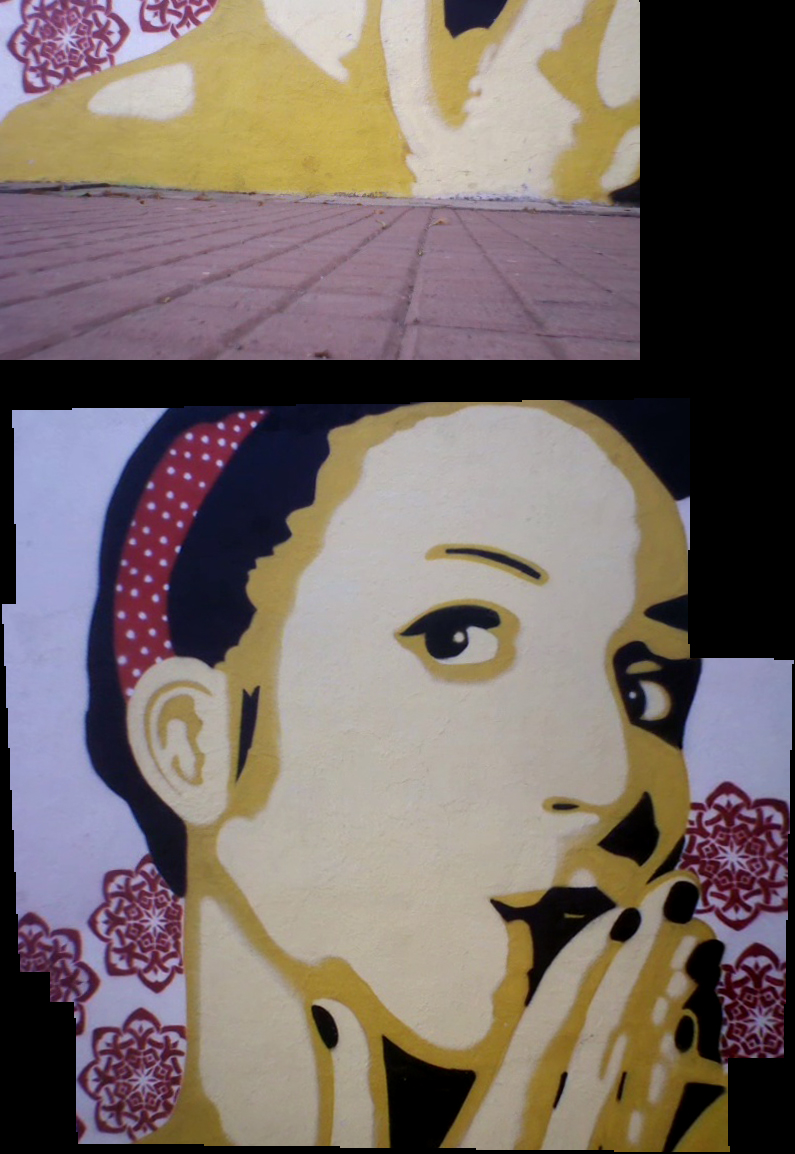
\includegraphics[width=\linewidth]{figures/sac3/uniform_sampled/photoshop.jpg}
\caption{Photoshop Result}
\end{subfigure}
\caption{Output of state of the art photo stitchers on uniformly time
  sampled images. As time sampled images do not guarantee 
  coverage of the scene, the panorama is broken. The top portions do
  not belong at the right place (see Figure~\ref{fig:results_sac3})}
\label{fig:results_sac3_timesmapled}
\end{figure*}


\begin{figure*}[htb!]
\centering

\includegraphics[width=0.19\linewidth]{figures/sac3/selected/1.jpg}
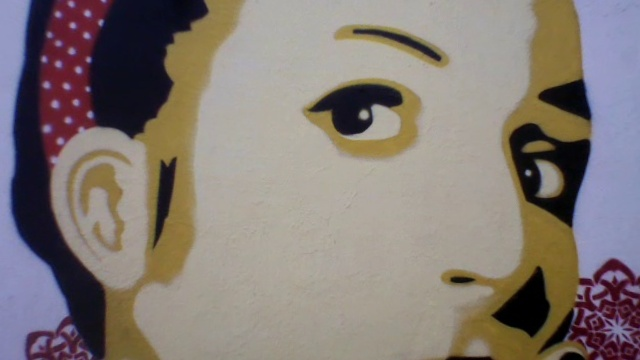
\includegraphics[width=0.19\linewidth]{figures/sac3/selected/5.jpg}
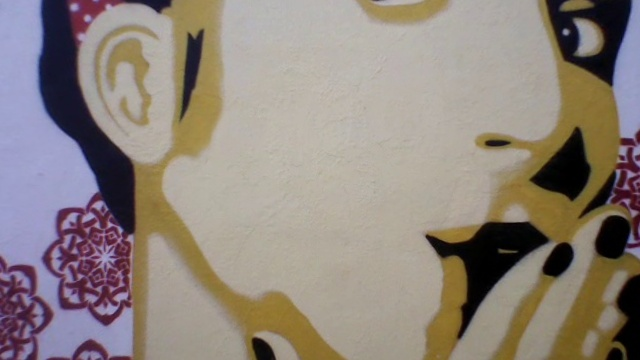
\includegraphics[width=0.19\linewidth]{figures/sac3/selected/4.jpg}
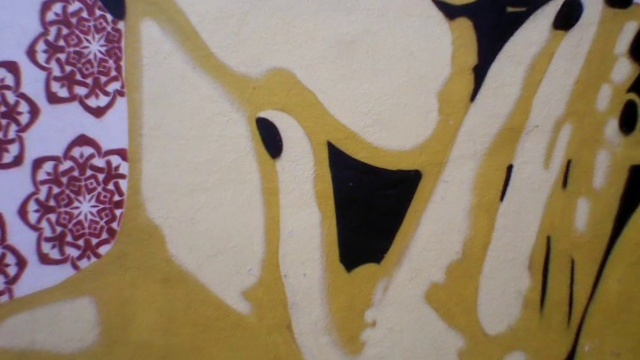
\includegraphics[width=0.19\linewidth]{figures/sac3/selected/2.jpg}

\includegraphics[width=0.19\linewidth]{figures/sac3/selected/3.jpg}
\caption{Salient image selection from the set of approximately 9000
  images using positional information.}
\label{fig:selected_sac3}
\end{figure*}


\begin{figure*}
\centering
\begin{subfigure}[b]{0.3\textwidth}
\centering
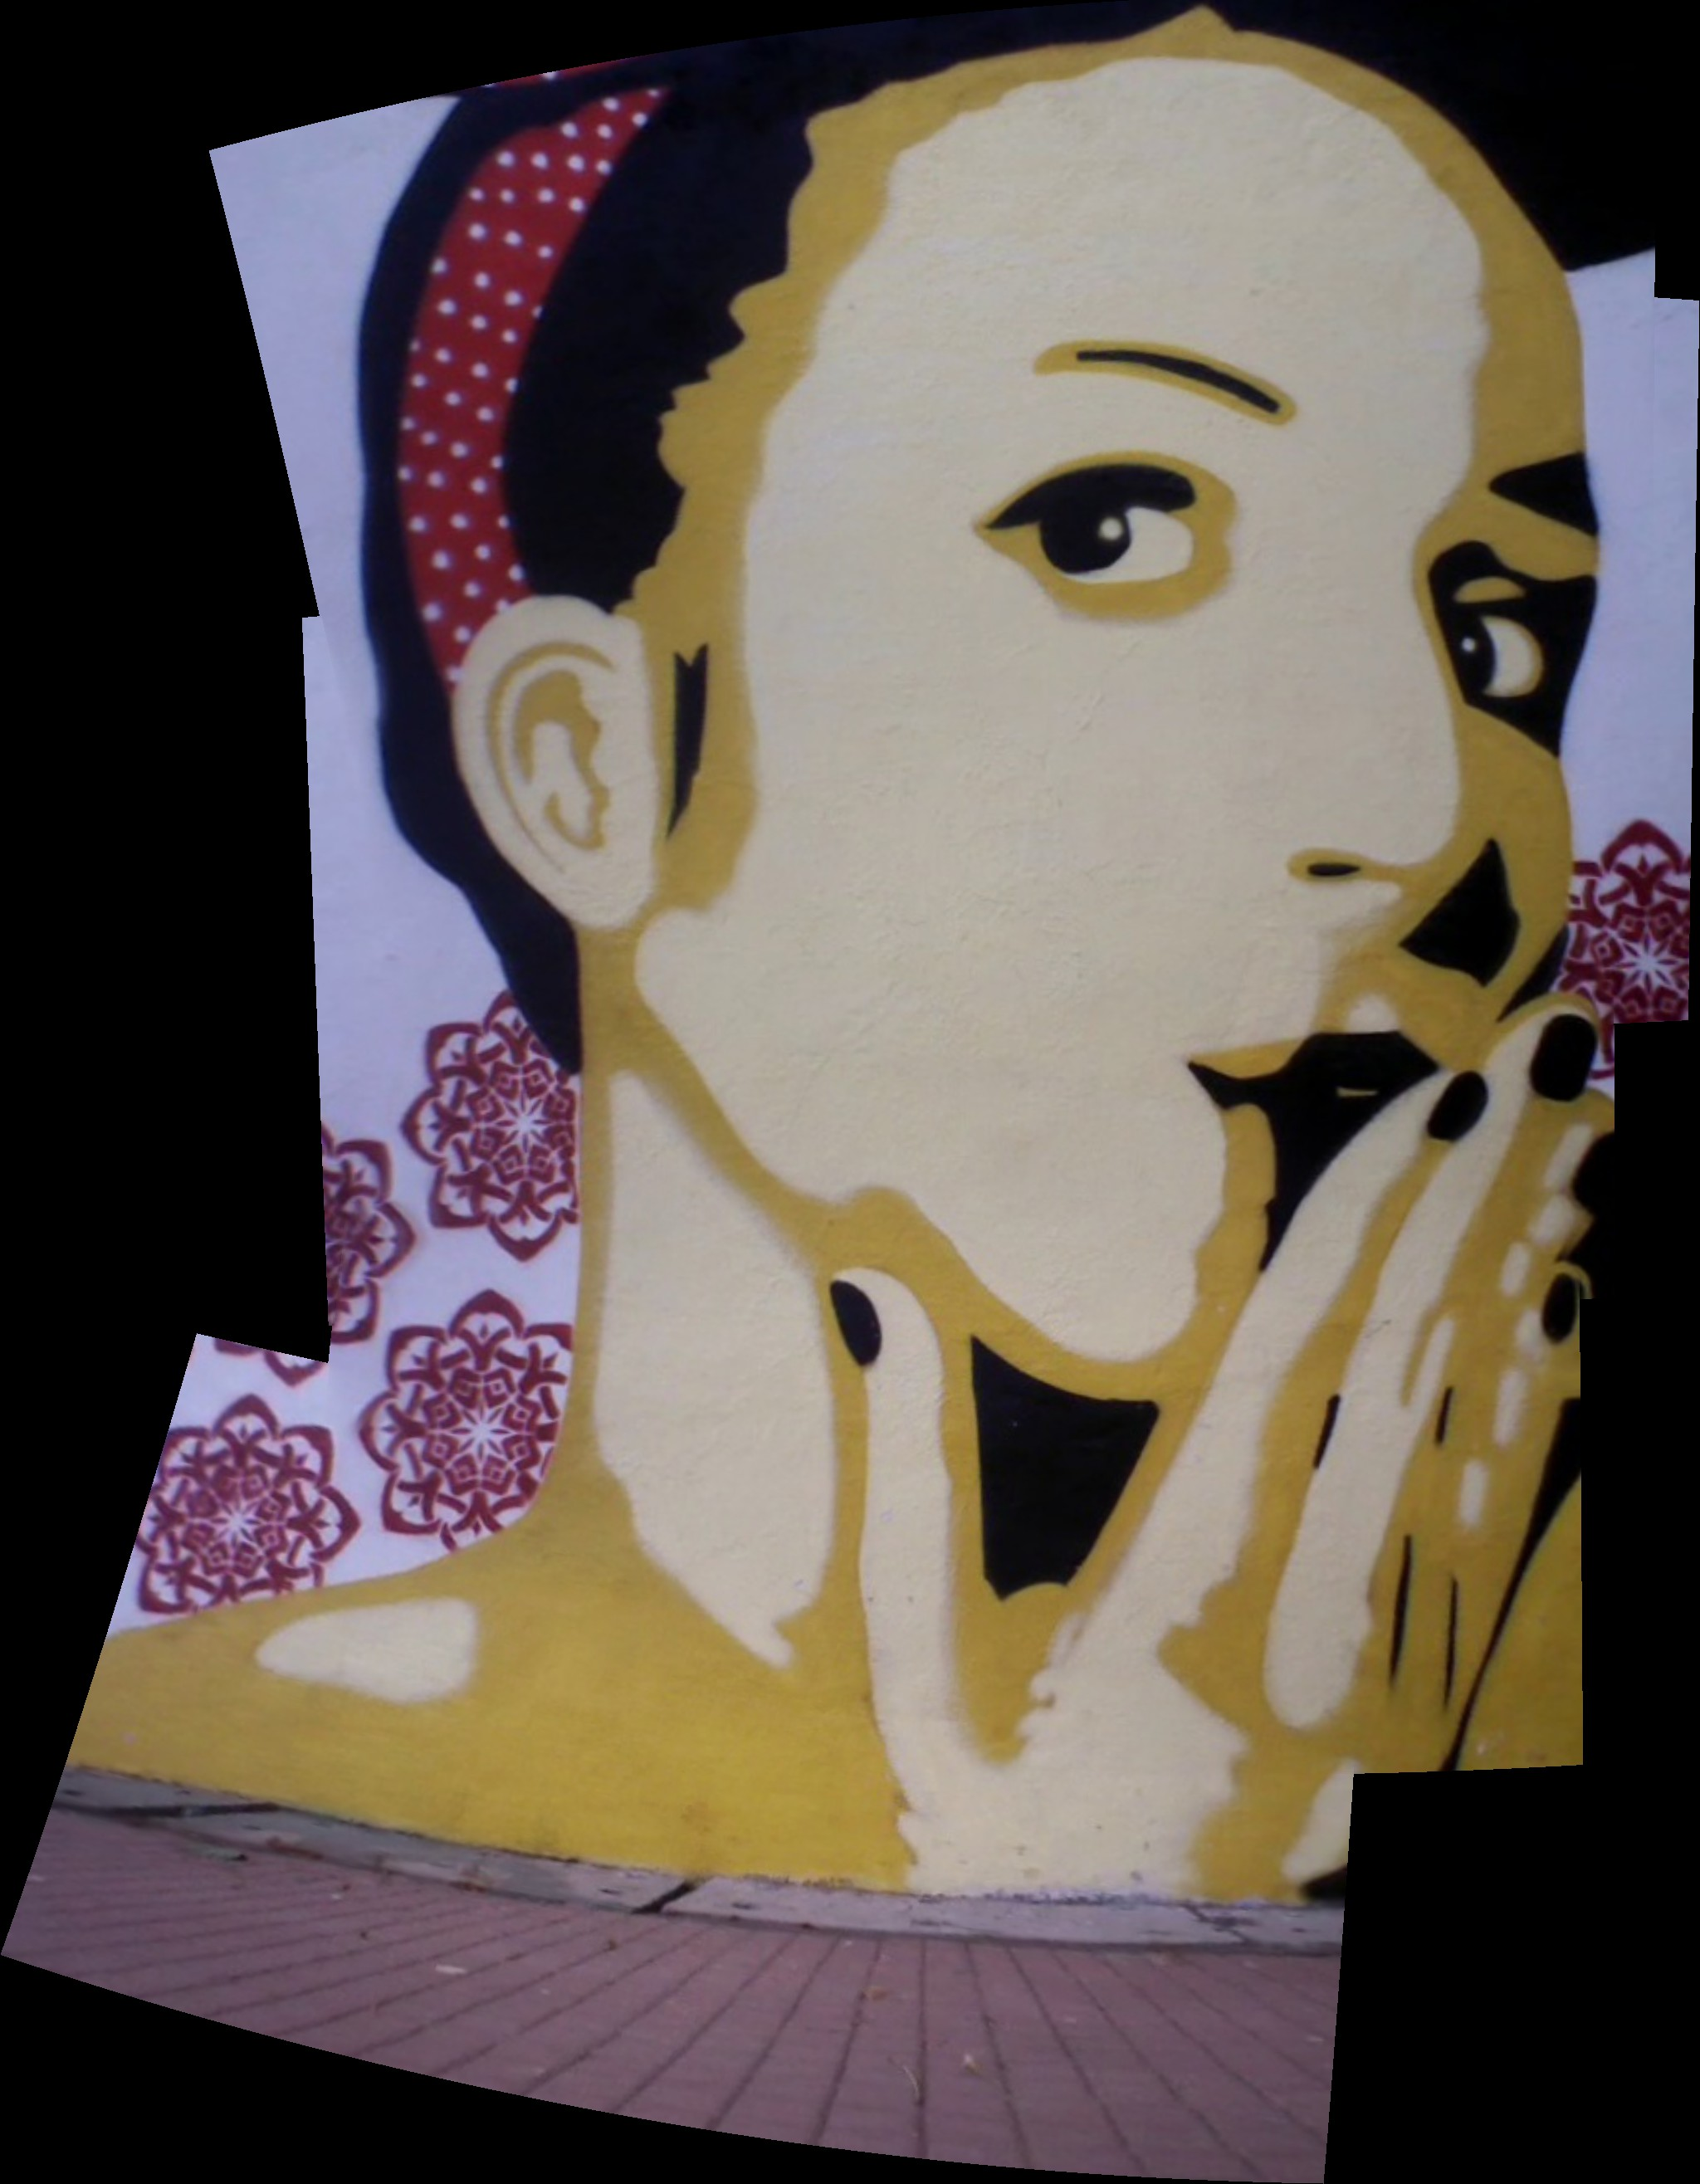
\includegraphics[width=\linewidth]{figures/sac3/autostitch.jpg}
\caption{Autostitch Result}
\end{subfigure}
\begin{subfigure}[b]{0.3\textwidth}
\centering
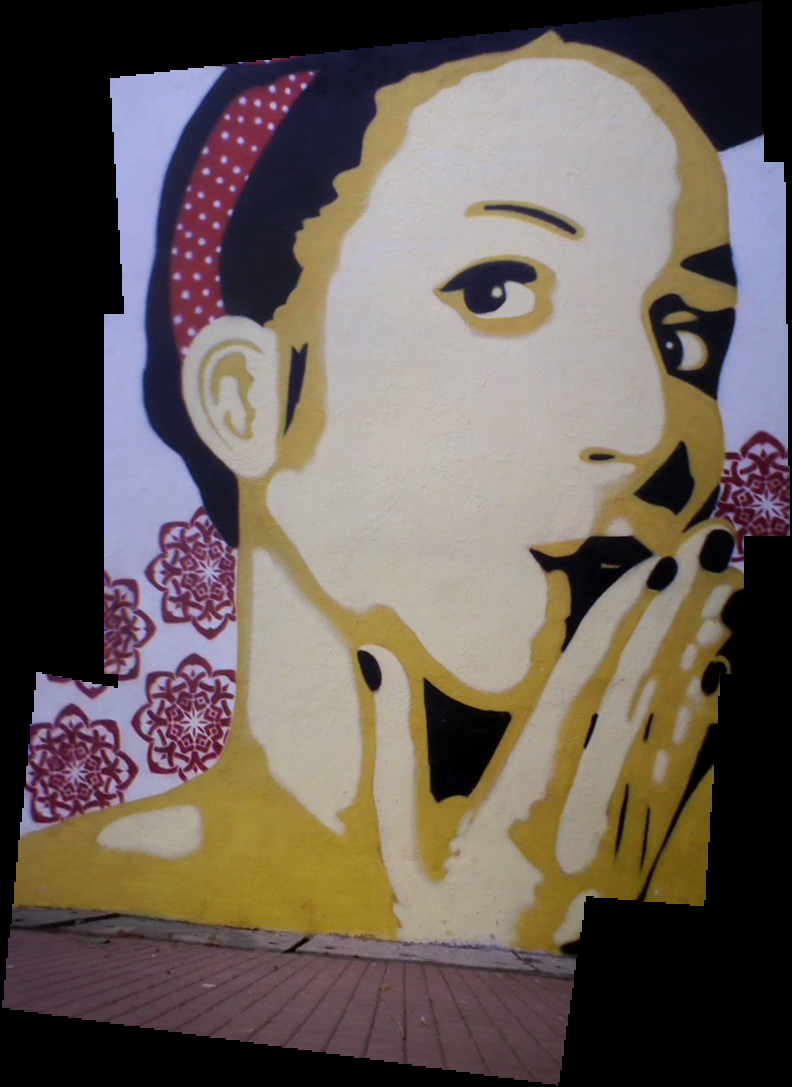
\includegraphics[width=\linewidth]{figures/sac3/photoshop.jpg}
\caption{Photoshop Result}
\end{subfigure}
\begin{subfigure}[b]{0.3\textwidth}
\centering
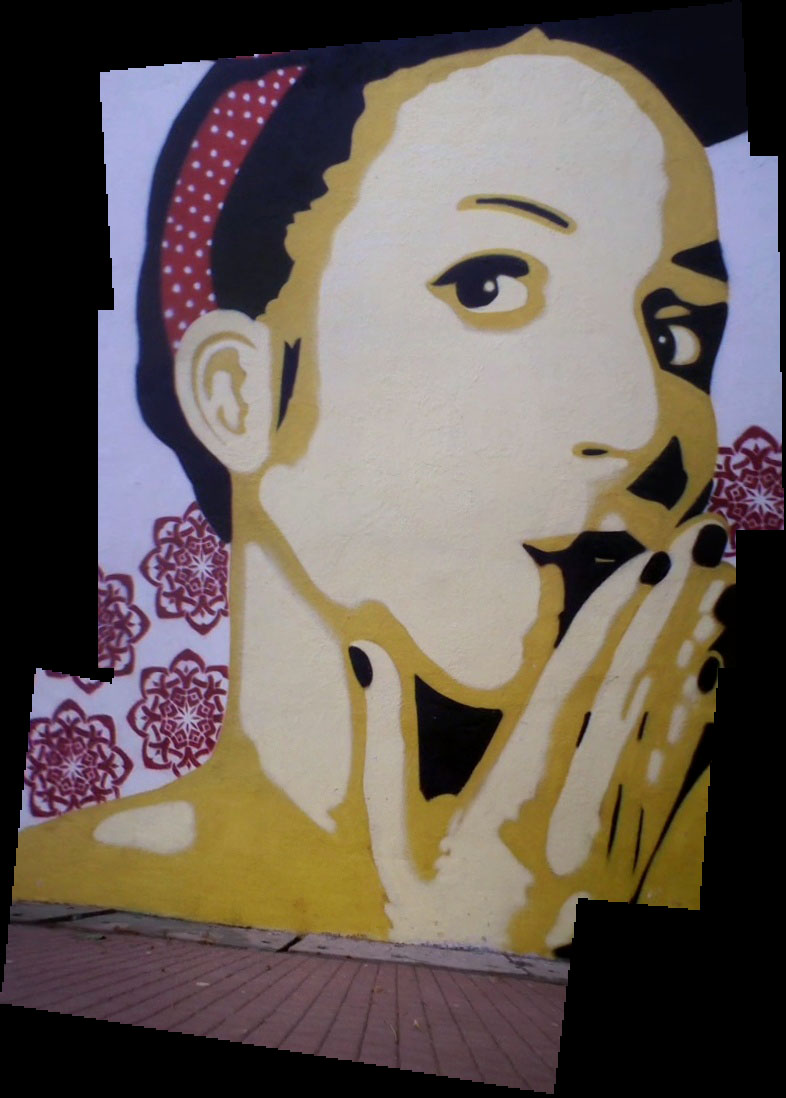
\includegraphics[width=\linewidth]{figures/sac3/our_result.jpg}
\caption{Our Result}
\end{subfigure}
\caption{When salient images are given to Autostich and Photoshop, a
  video can be used to create a panaromic mosaic provided there is no
  dead space. We also show the results from our stitching algorithm.}
\label{fig:results_sac3}
\end{figure*}

In summary, this experiment provides evidence to show that (a) our
saliency selection algorithm is reasonable and (b) our stitching
results are comparable to that of Autostitch for the kind of scenes
considered.

\subsection{Indoor Imagery with Dead Space} 

Our next selection of experiments were conducted in an indoor
environment with some natural light.  The input stream had about 4300
images. The selection algorithm pruned the video into N=4 images. A
sample of the selected images are seen in Figure~\ref{fig:idc_selected}

\begin{figure}
\centering

\includegraphics[width=0.22\linewidth]{figures/idc_indoor/selected/1.jpg}

\includegraphics[width=0.22\linewidth]{figures/idc_indoor/selected/2.jpg}

\includegraphics[width=0.22\linewidth]{figures/idc_indoor/selected/3.jpg}

\includegraphics[width=0.22\linewidth]{figures/idc_indoor/selected/4.jpg}
\caption{Pruned images from a video of an indoor scene.}
\label{fig:idc_selected}
\end{figure}

There were two disconnected components in the resulting graph.
Autostitch was unable to produce any reasonable output as seen in
Figure~\ref{fig:idc_indoor_comparison}.  The ground truth can be seen
in Figure~\ref{fig:idc_indoor_groundtruth}.  One can see a better
orthographic view of the posters in a composite manner.


\begin{figure}[p]

\includegraphics[width=\linewidth]{figures/idc_indoor/groundtruth.jpg}
\caption{Ground truth of the indoor scene.  There is a substantial gap
  in between the two posters, and this dead space confuses state of the
  art stitchers since they do not find features.}
\label{fig:idc_indoor_groundtruth}
\end{figure} 

Figure \ref{fig:idc_indoor_comparison} shows the comparison of outputs of state
of the art stitchers with output of our algorithm. 

\begin{figure*}
\begin{subfigure}[b]{0.45\textwidth}

\includegraphics[width=\linewidth]{figures/idc_indoor/autostitch.jpg}
\caption{Autostitch Result}
\end{subfigure}
\begin{subfigure}[b]{0.45\textwidth}

\includegraphics[width=\linewidth]{figures/idc_indoor/photoshop.jpg}
\caption{Photoshop Result}
\end{subfigure}
\begin{subfigure}[b]{\textwidth}

\includegraphics[width=\linewidth]{figures/idc_indoor/our_result.jpg}
\caption{Our Result}
\end{subfigure}
\caption{Comparison of outputs of Autostich, Photoshop and our stitching
algorithm on an indoor scene. Only our
algorithm is able to show a complete super-panorama; state-of-the art
stitchers can produce only one mini-panorama.}
\label{fig:idc_indoor_comparison}
\end{figure*}

One can see a better orthographic view of the posters in a composite
manner. Autostitch was unable to produce any reasonable output as seen in
Figure \ref{fig:idc_indoor_comparison}.

\subsection{Outdoor Imagery with Dead Space}
Our next set of experiments were conducted in an outdoor environment. The  
input stream had about 12000 images. The selection algorithm pruned the video
into N=30 images. A sample of the selected images are seen in Figure
\ref{fig:green_red_selected}.

\begin{figure}
\centering

\includegraphics[width=0.19\linewidth]{figures/green_red/selected/1.jpg}
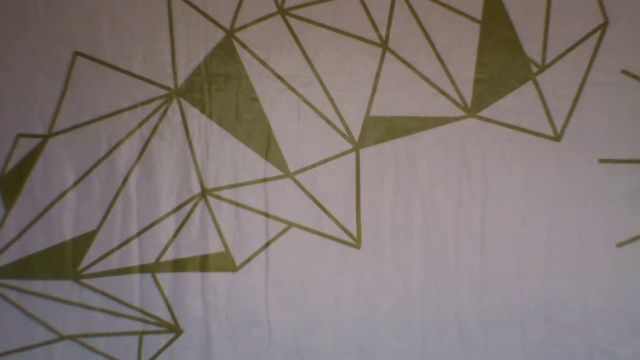
\includegraphics[width=0.19\linewidth]{figures/green_red/selected/2.jpg}

\includegraphics[width=0.19\linewidth]{figures/green_red/selected/3.jpg}
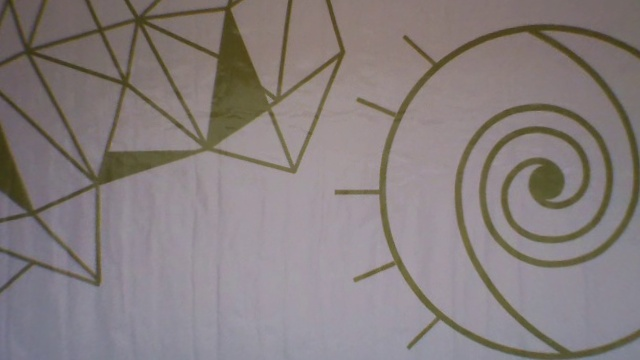
\includegraphics[width=0.19\linewidth]{figures/green_red/selected/4.jpg}
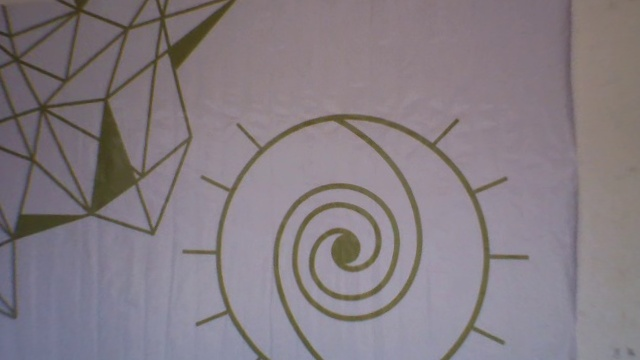
\includegraphics[width=0.19\linewidth]{figures/green_red/selected/5.jpg}
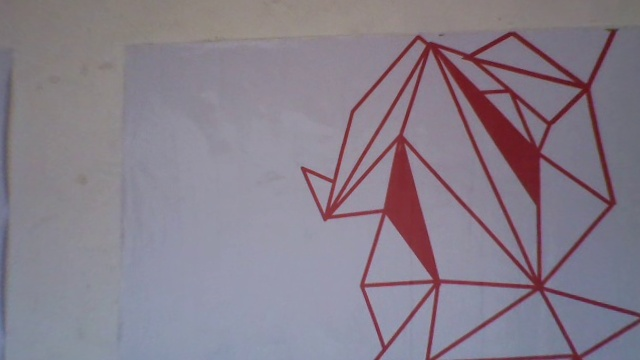
\includegraphics[width=0.19\linewidth]{figures/green_red/selected/6.jpg}

\includegraphics[width=0.19\linewidth]{figures/green_red/selected/7.jpg}
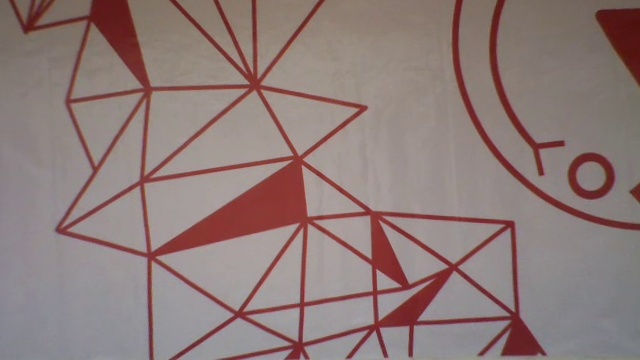
\includegraphics[width=0.19\linewidth]{figures/green_red/selected/8.jpg}

\includegraphics[width=0.19\linewidth]{figures/green_red/selected/9.jpg}
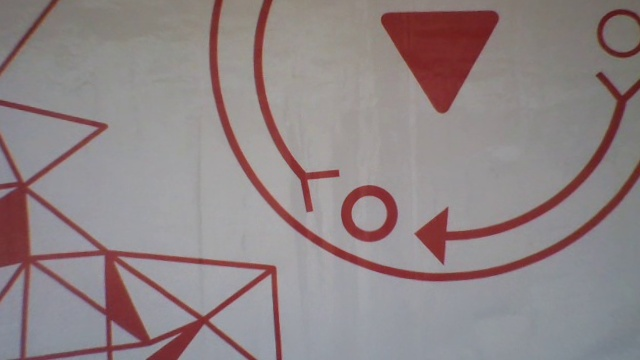
\includegraphics[width=0.19\linewidth]{figures/green_red/selected/10.jpg}
\caption{Sample selected images of outdoor scene by our algorithm.}
\label{fig:green_red_selected}
\end{figure}

The ground truth of outdoor scene can be seen in Figure
\ref{fig:green_red_groundtruth}.

\begin{figure}
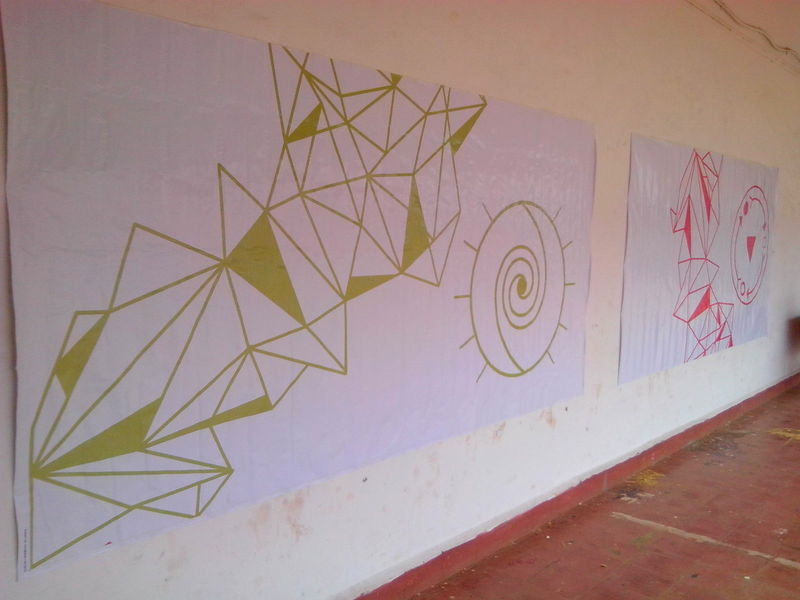
\includegraphics[width=\linewidth]{figures/green_red/groundtruth.jpg}
\caption{Ground truth of the outdoor scene captured by quadcopter. There is
visible gap in between two posters which will cause problems for state of the art
stitchers.}
\label{fig:green_red_groundtruth}
\end{figure}


\begin{figure*}
\begin{subfigure}[b]{0.45\textwidth}
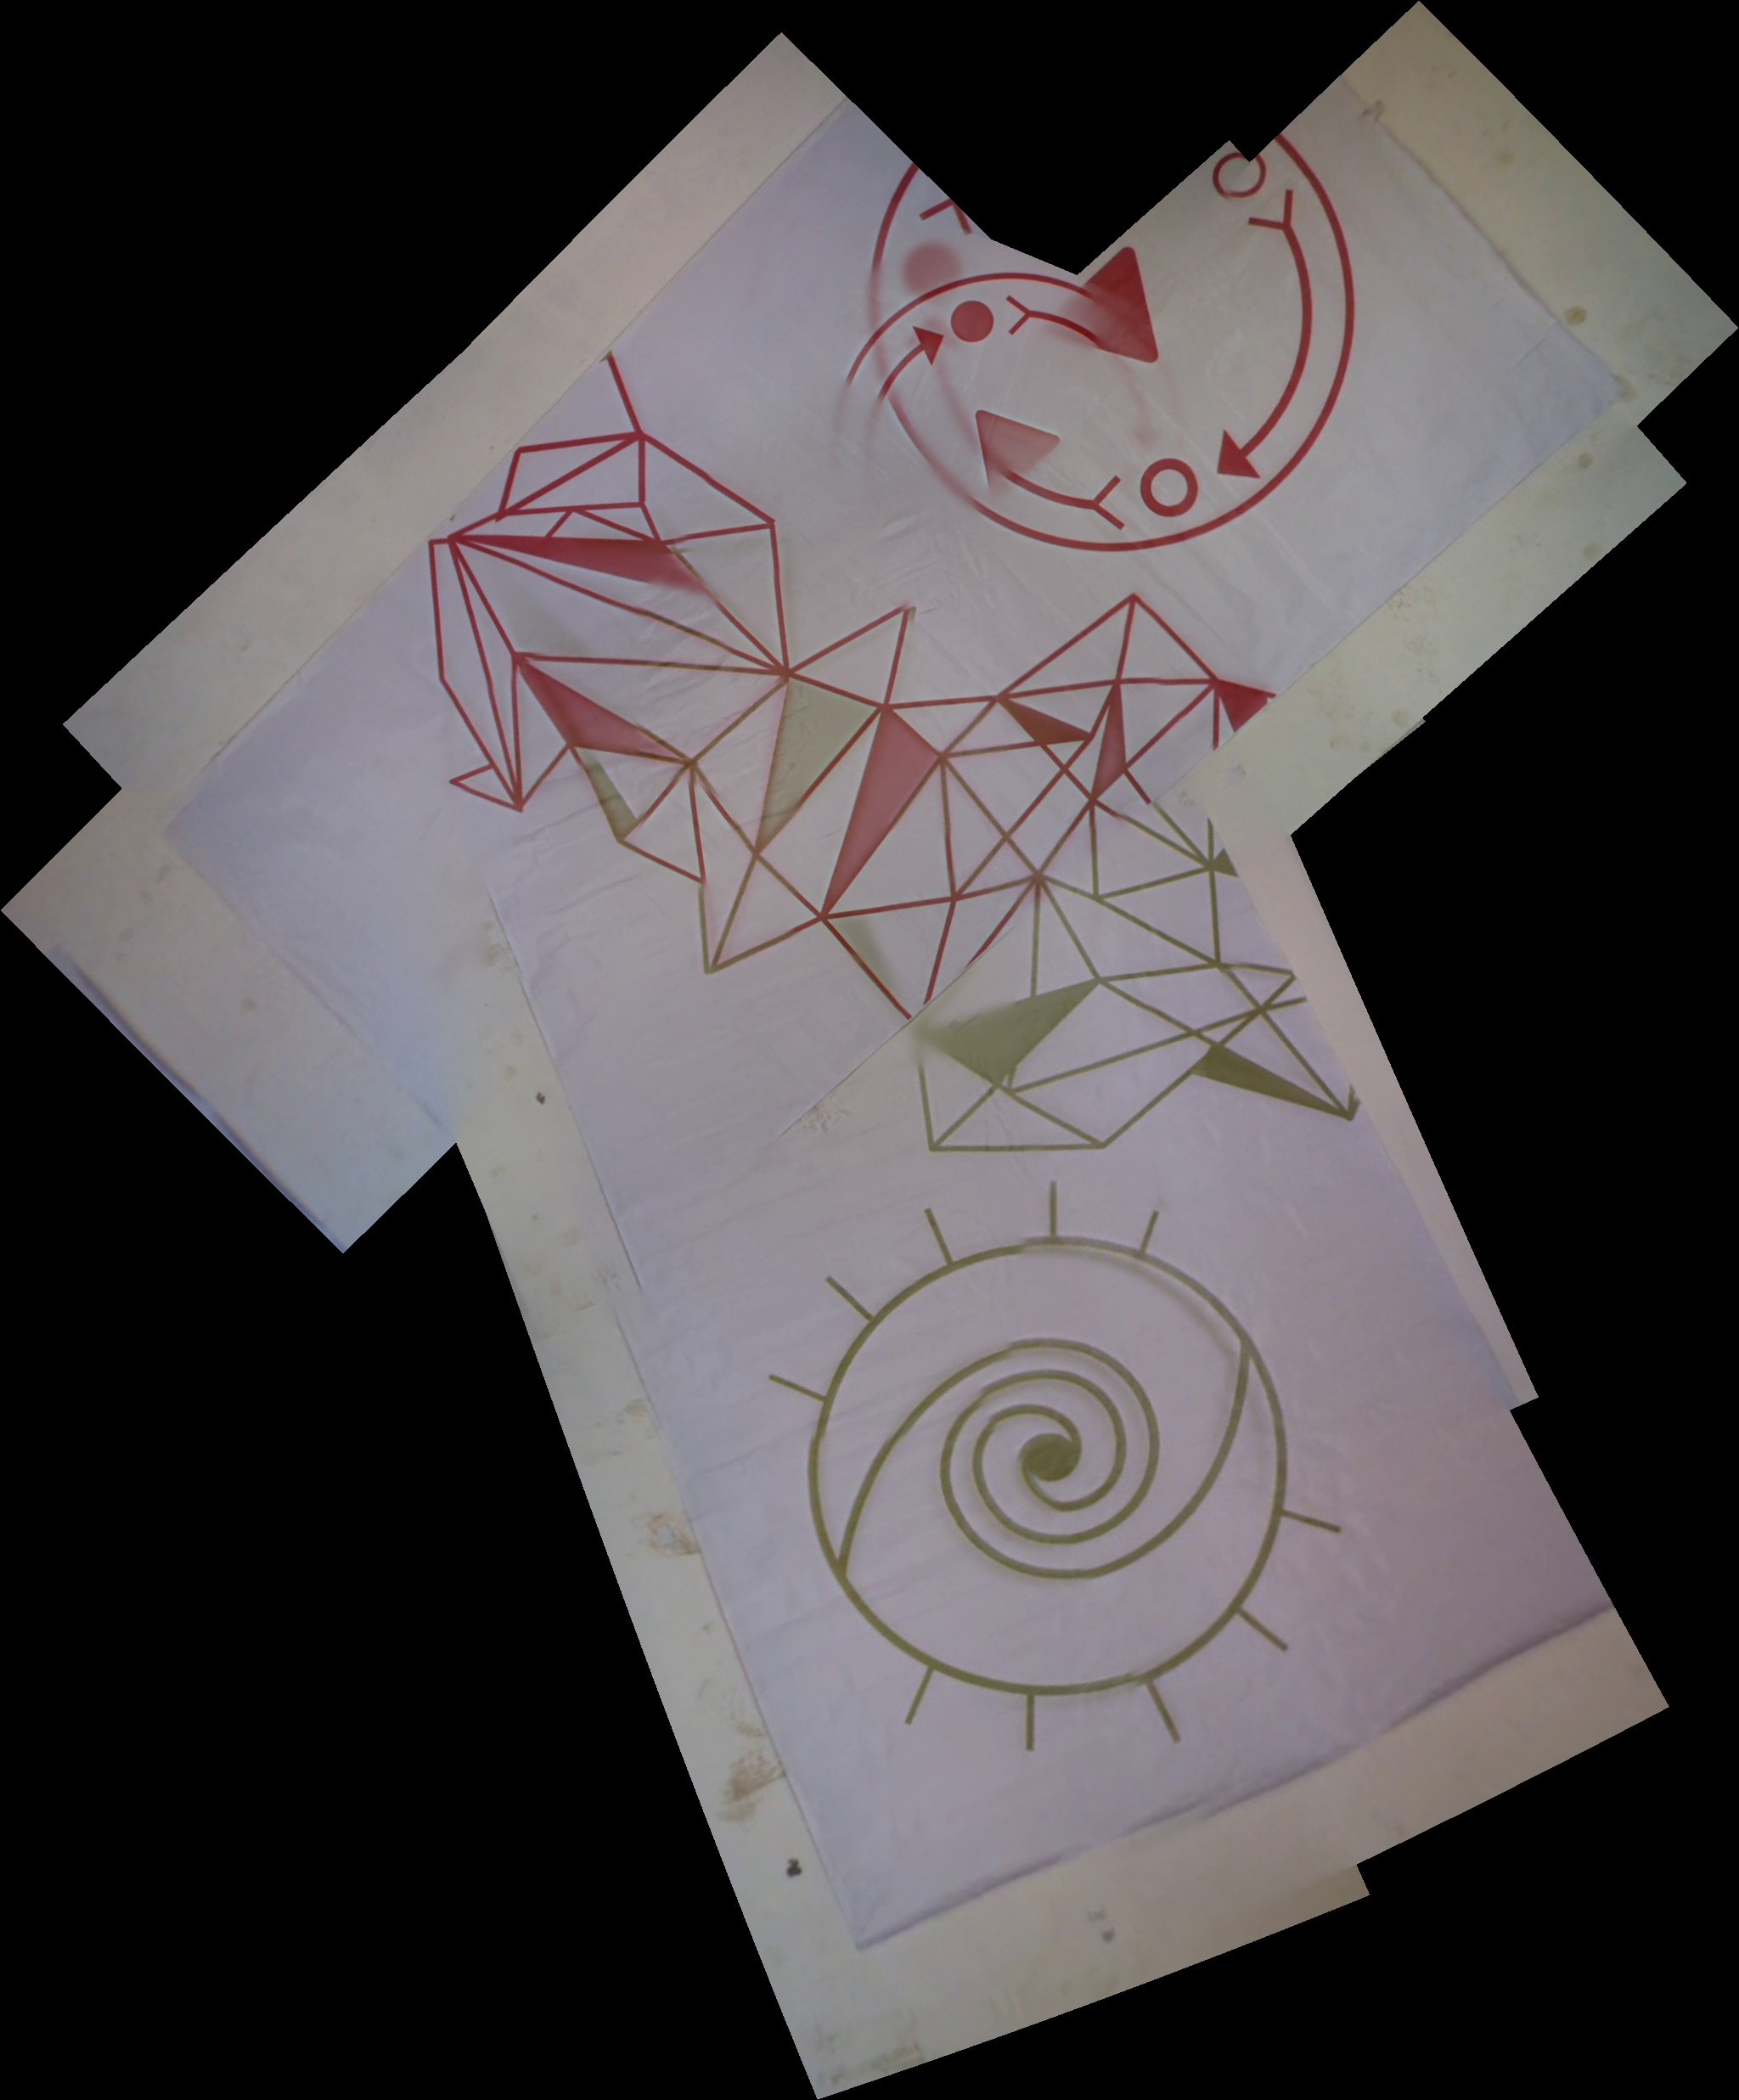
\includegraphics[width=\linewidth]{figures/green_red/autostich.jpg}
\caption{Autostitch Result}
\end{subfigure}
\begin{subfigure}[b]{0.45\textwidth}
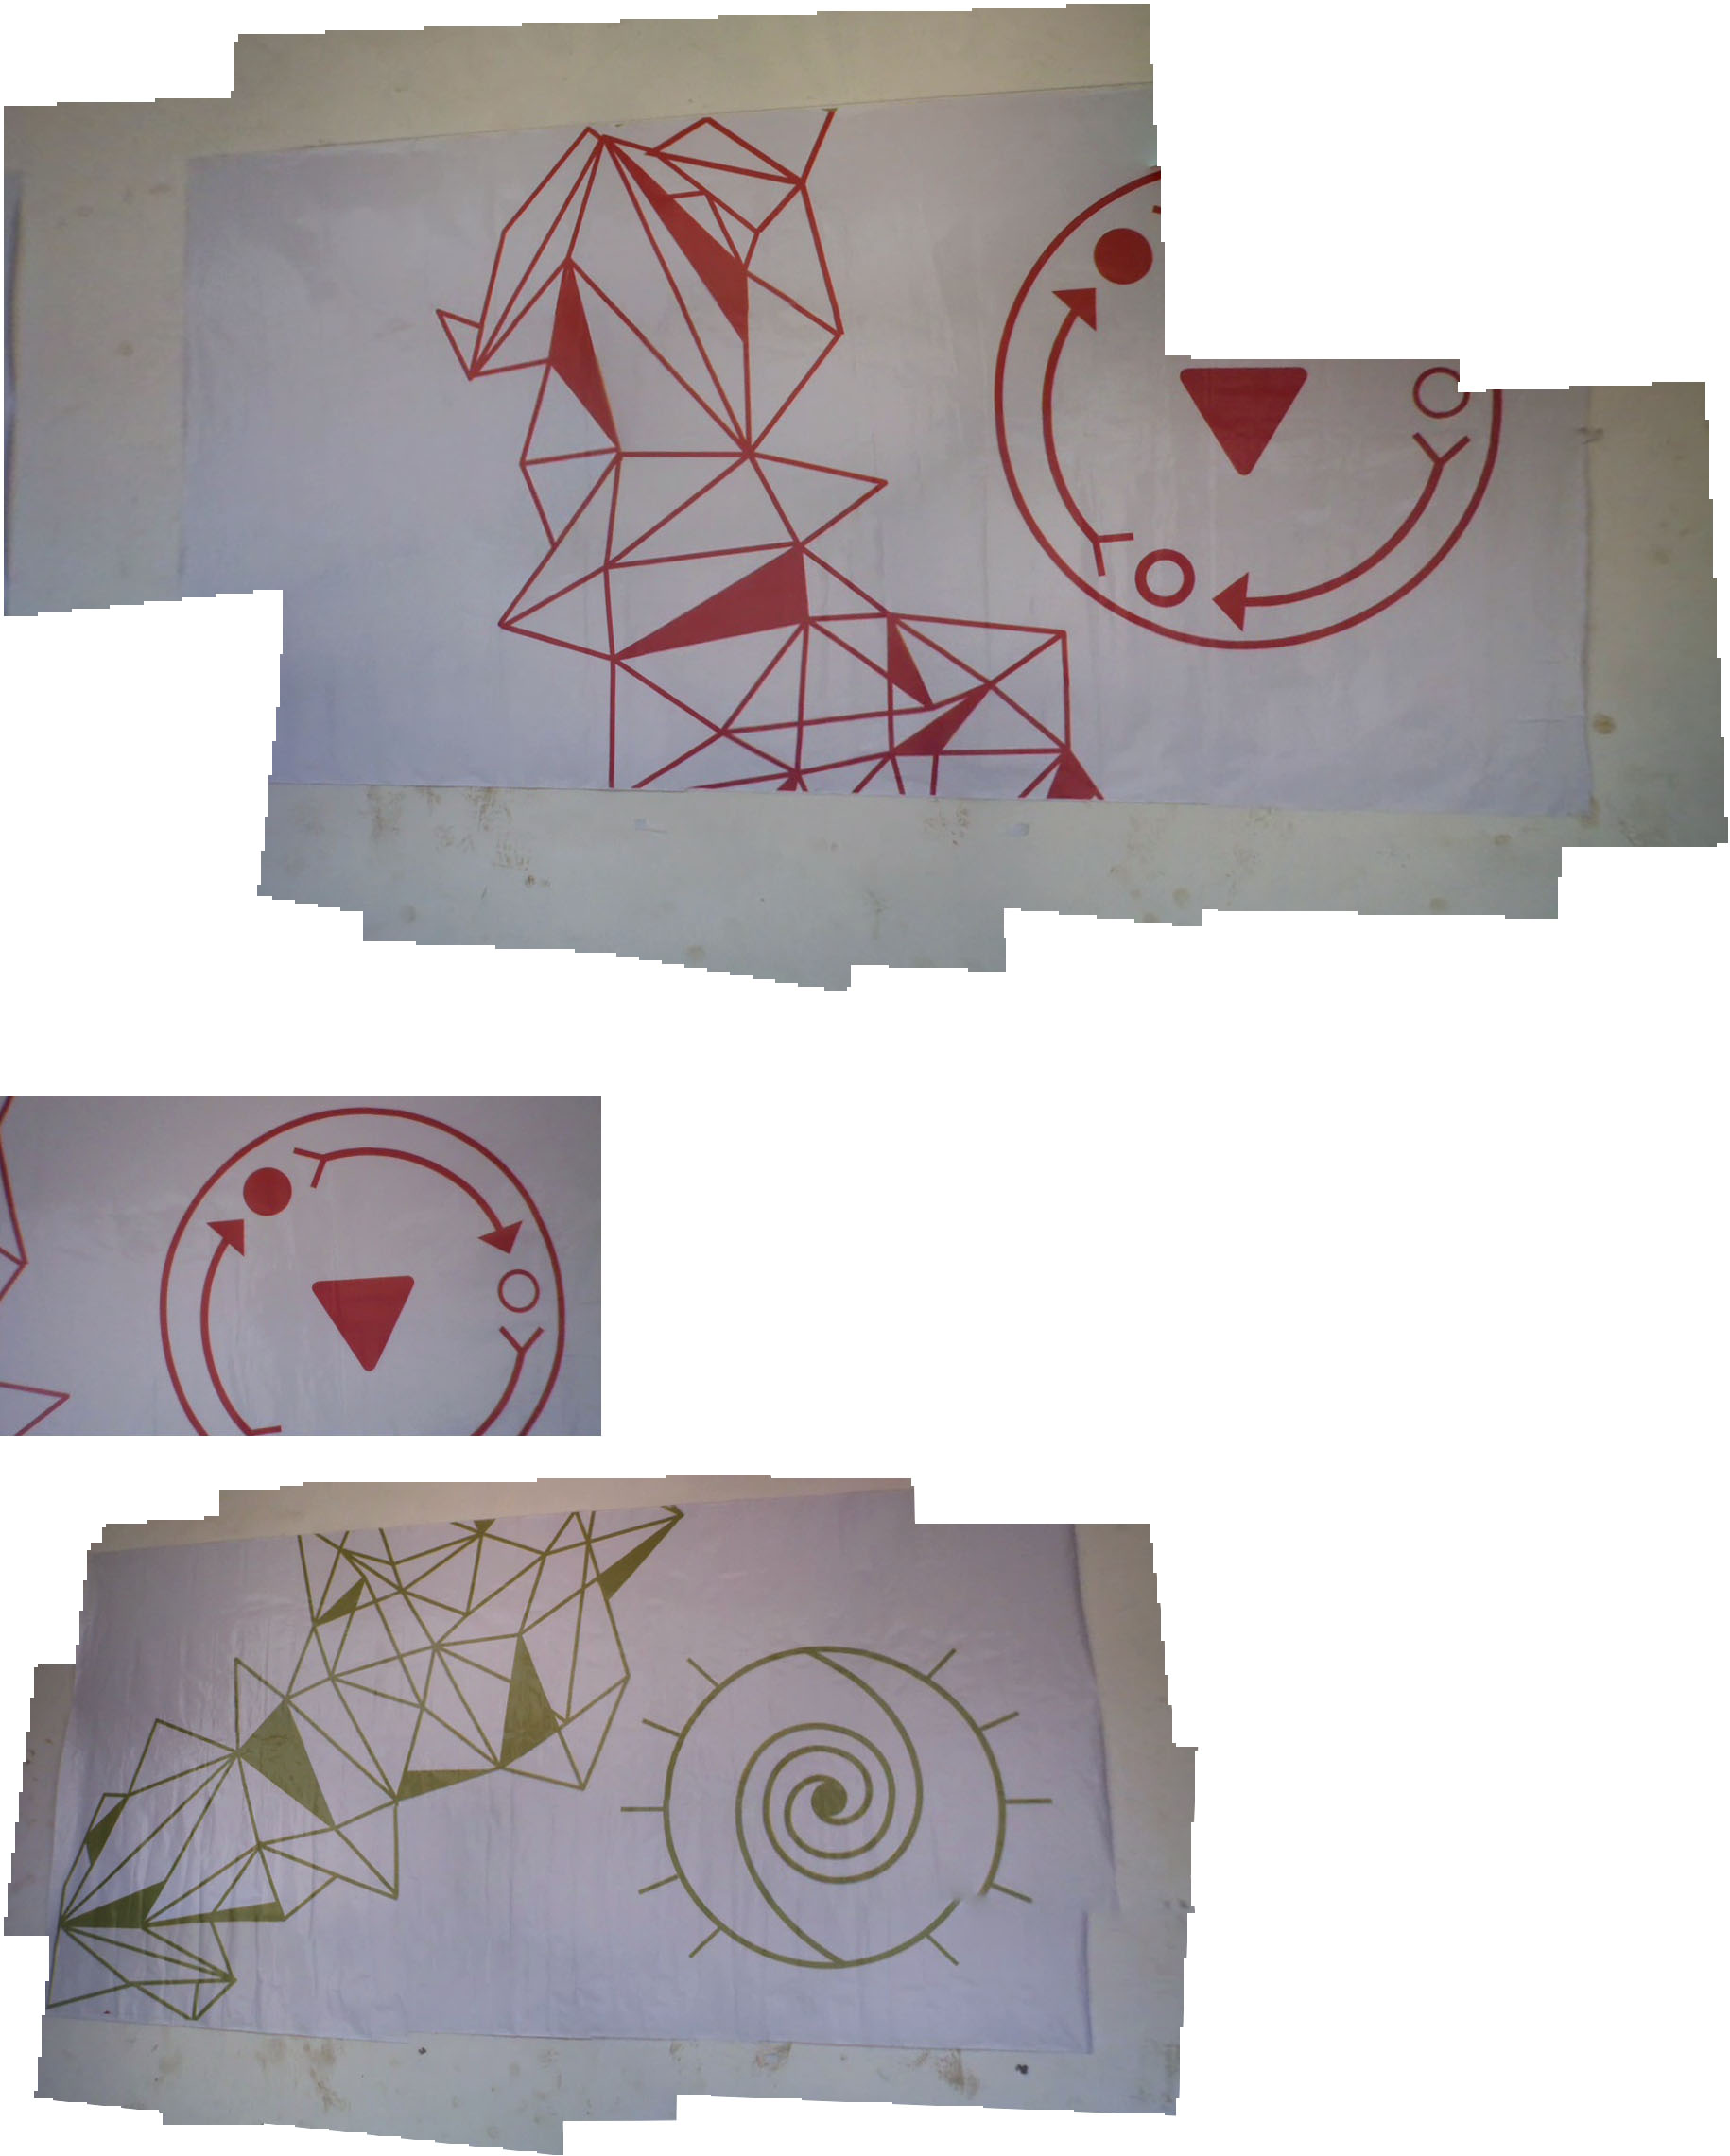
\includegraphics[width=\linewidth]{figures/green_red/photoshop_output.jpg}
\caption{Photoshop Result}
\end{subfigure}\\
\begin{subfigure}[b]{\textwidth}
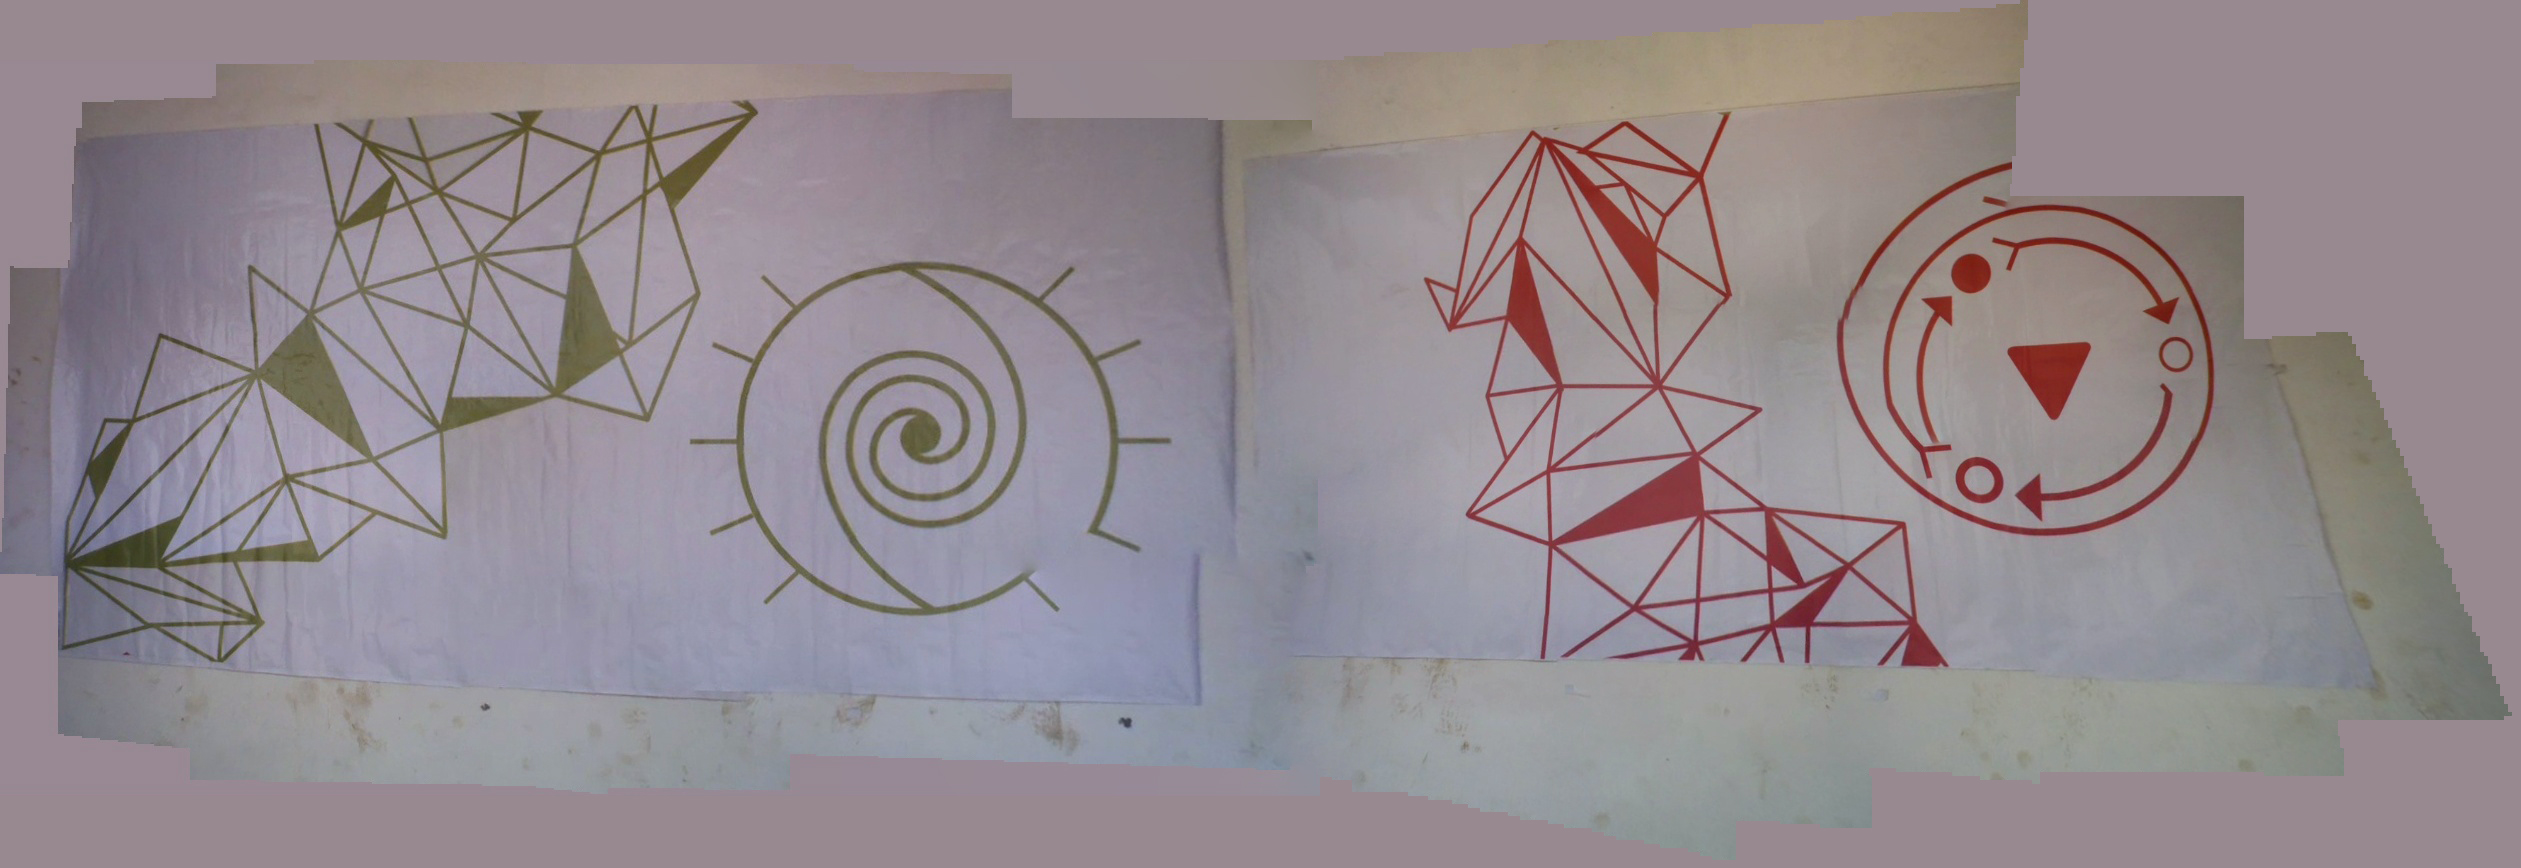
\includegraphics[width=\linewidth]{figures/green_red/our_result.jpg}
\caption{Our Result}
\end{subfigure}
\caption{Comparison of outputs of Autostich, Photoshop and our stitching
algorithm on the images selected of outdoor scene by our algorithm. Only our
output is able to shows individual panoramas at their respective location
approximately}
\label{fig:green_red_comparison}
\end{figure*}

Figure \ref{fig:green_red_comparison} shows the comparison of outputs of
state of the art stitchers with output of our algorithm.

\section{Concluding remarks}

% pleasing composite doesn't make scene.  
In this paper, we have defined a new problem, that of computing a
mosaic of a planar scene with vacant spaces.  Vacant space relates to images
in an input stream where there are not enough features for traditional
mosaicing algorithms to estimate geometric warps to align the images.

Our solution to this problem is to use an autonomous quadcopter which
is capable of taking pictures.  The quadcopter has an inertial
measurement unit that is capable of outputting approximate
positions. Using this positional information, our algorithm selects an
``interesting'' subset of the video imagery.  This subset consists of
pictures taken with a moving camera; we reduce the resulting
problem of computing a mosaic by reduction to the stereo problem.  Our
method works on both indoor and outdoor scenes.

{\bf Future work} Controlling a consumer-focused inexpensive
quadcopter can be problematic; for instance the quadcopter could have
severe yaw and roll.  Vision based algorithms to control such
quadcopters might be quite useful.


\bibliographystyle{ieee}
\bibliography{egbib}
\end{document}
